
%http://www.latextemplates.com/template/masters-doctoral-thesis

\documentclass[11pt, a4paper, oneside]{Thesis}
\graphicspath{{./Figures/}}
% The svg package is gone: it ran Inkscape through shell-escape on every compile,
% which cost more than the Overleaf free-plan timeout allows and does not work under
% Tectonic. The two SVG figures are pre-converted to PDF in Figures/ and included with
% \includegraphics. README.md gives the rsvg-convert command that regenerates them.
\usepackage[square, numbers, comma, sort&compress]{natbib} 
\usepackage{array, booktabs, multirow, longtable}
\usepackage{tabularx}
% Ragged-right X column: prose tables set badly when justified in narrow columns.
\usepackage{xltabular} % X columns inside a longtable, so wide tables can break across pages
\newcolumntype{L}{>{\raggedright\arraybackslash}X}
\newcolumntype{P}[1]{>{\raggedright\arraybackslash}p{#1}} % ragged fixed-width column
\usepackage{xurl} % long reference URLs break instead of running into the margin
\usepackage{enumitem} % roman-numeral list labels in the Intellectual Property Statement
\usepackage{color}
\definecolor{dkgreen}{rgb}{0,0.6,0}
\definecolor{gray}{rgb}{0.5,0.5,0.5}
\definecolor{mauve}{rgb}{0.58,0,0.82}

\lstset{frame=tb,
  language=Java,
  aboveskip=3mm,
  belowskip=3mm,
  showstringspaces=false,
  columns=flexible,
  basicstyle={\small\ttfamily},
  numbers=none,
  numberstyle=\tiny\color{gray},
  keywordstyle=\color{blue},
  commentstyle=\color{dkgreen},
  stringstyle=\color{mauve},
  breaklines=true,
  breakatwhitespace=true,
  tabsize=3
}

\newcommand{\todo}[1]{\textcolor{red}{(TODO) #1}}
\hypersetup{urlcolor=black, colorlinks=true}

%----------------------------------------------------------------------------------------
%	YOUR DETAILS -- EDIT THIS BLOCK, AND ONLY THIS BLOCK
%
%	These override the empty defaults set in Thesis.cls (lines 190-219).
%	Everything else -- title page, declaration, PDF metadata -- reads from here,
%	so you never have to edit those files by hand.
%	Replace every [SQUARE BRACKET] placeholder before submitting.
%----------------------------------------------------------------------------------------

\thesistitle{Pharmacy Capacity and the NHS 60-Day Clinical-Trial Set-up Target}
\authors{Kachanon Lertdamrongwong}
\newcommand{\studentid}{14287892}
\supervisor{Ahmed Kheiri}
\degree{MSc Business Analytics: Operational Research and Risk Analysis}
\university{The University of Manchester}
\department{Alliance Manchester Business School}
\faculty{Faculty of Humanities}
\subject{Business Analytics}
\keywords{clinical trial set-up; pharmacy capacity; NHS research delivery; integer programming; goal programming; queueing theory}
\newcommand{\subdate}{September 2026} % Submission date shown on the title page

%----------------------------------------------------------------------------------------

\title{\ttitle} % Defines the thesis title - don't touch this
\begin{document}
\frontmatter
\setstretch{1.3} % Line spacing of 1.3
\fancyhead{} % Clears all page headers and footers
\rhead{\thepage} % Sets the right side header to show the page number
\lhead{} % Clears the left side page header
\pagestyle{fancy} % Finally, use the "fancy" page style to implement the FancyHdr headers



\newcommand{\HRule}{\rule{\linewidth}{0.5mm}} % New command to make the lines in the title page
\hypersetup{pdftitle={\ttitle}}
\hypersetup{pdfsubject=\subjectname}
\hypersetup{pdfauthor=\authornames}
\hypersetup{pdfkeywords=\keywordnames}


%-----------------
%	FIRST PAGES
%-----------------

% All values on this page come from the details block at the top of main.tex.
% Do not hardcode names here -- edit main.tex instead.

\begin{titlepage}
\begin{center}

% Drop your university logo in as Figures/logo.png (or logo.jpg) and it appears
% automatically. With no logo file present the page still compiles cleanly.
\IfFileExists{Figures/logo.png}{%
  \begin{figure}[htbp]
  \centering
  \includegraphics[width=0.24\textwidth]{logo.png}
  \end{figure}
}{%
  \IfFileExists{Figures/logo.jpg}{%
    \begin{figure}[htbp]
    \centering
    \includegraphics[width=0.24\textwidth]{logo.jpg}
    \end{figure}
  }{}%
}

\textsc{\LARGE \univname}\\[0.7cm]
\HRule \\[0.4cm]
{\huge \bfseries \ttitle}\\[0.4cm]
\HRule \\[0.7cm]
{\LARGE \bfseries \authornames}\\[0.4cm]
{\LARGE \studentid}\\[1cm]
{\large \bfseries Supervisor}\\[0.4cm]
{\large \bfseries \supname}\\[1cm]
\large \textit{A thesis submitted in fulfilment of the requirements\\ for the degree of \degreename}\\[0.3cm]
\textit{in the}\\[0.4cm]
\facname \\
\deptname\\[1cm]
{\large \subdate}\\[4cm]
\vfill
\end{center}
\end{titlepage}



\Declaration{

\addtocontents{toc}{\vspace{1em}}  % Add a gap in the Contents, for aesthetics

I, \textbf{\authornames}, hereby declare that this thesis entitled, \textbf{``\ttitle"}, is all my own work, except as indicated in the text.

The report has not been accepted for any degree and it is not being submitted currently in candidature for any degree or other reward.

 
 
Signed:\\
\rule[1em]{25em}{0.5pt}  % This prints a line for the signature
 
Date:\\
\rule[1em]{25em}{0.5pt}  % This prints a line to write the date
}
\clearpage  % Declaration ended, now start a new page

%% ----------------------------------------------------------------

 
 
 

\btypeout{Intellectual Property Statement}
\addtotoc{Intellectual Property Statement}
\thispagestyle{plain}
\begin{center}{\huge\bf Intellectual Property Statement\par}\end{center}
\vspace{1em}

\begin{enumerate}[label=\roman*.]

\item The author of this dissertation (including any appendices and/or schedules to this dissertation) owns certain copyright or related rights in it (the `Copyright') and s/he has given The University of Manchester certain rights to use such Copyright including for administrative purposes.

\item Copies of this dissertation, either in full or in extracts and whether in hard or electronic copy, may be made \textbf{only} in accordance with the Copyright, Designs and Patents Act 1988 (as amended) and regulations issued under it or, where appropriate, in accordance with licensing agreements which the University has entered into. This page must form part of any such copies made.

\item The ownership of certain Copyright, patents, designs, trademarks and other intellectual property (the ``Intellectual Property'') and any reproductions of works in the dissertation, for example graphs and tables (``Reproductions''), which may be described in this dissertation, may not be owned by the author and may be owned by third parties. Such Intellectual Property and Reproductions cannot and must not be made available for use without the prior written permission of the owner(s) of the relevant Intellectual Property and/or Reproductions.

\item Further information on the conditions under which disclosure, publication and commercialisation of this dissertation, the Copyright and any Intellectual Property and/or Reproductions described in it may take place is available in the University IP Policy, in any relevant Dissertation restriction declarations deposited in the University Library, and The University Library's regulations.

\end{enumerate}

\clearpage

\addtotoc{Abstract}

\abstract{\addtocontents{toc}{\vspace{1em}}

\todo{Give a short (1 page) overview of the work. This should summarise (not advertise) your research project. After reading the abstract the reader should know what problem you are tackling, the techniques you are using, the results you have achieved.}
}

\clearpage

\setstretch{1.3}

\acknowledgements{\addtocontents{toc}{\vspace{1em}}

I would like to thank my supervisor, Professor Ahmed Kheiri, for his guidance and feedback throughout this dissertation.

My sincere thanks go to Christine Minnis and Jaya Shrivastava at LTHTR, who provided the data underpinning this work, patiently fulfilled every follow-up data request, met with me regularly throughout the project, and answered countless questions along the way. This dissertation was written with their pharmacy service in mind, and it would not have been possible without their time and openness.

I am also grateful to Kachanon Lertdamrongwong, who worked alongside me on this wider project and whose collaboration on the companion portfolio-selection model shaped much of the thinking behind this dissertation, and to Samantha for her support throughout. Thanks also to the wider LTHTR pharmacy and R\&I team for their engagement with this work.

}
\clearpage


%-------------------------------------------
%	LIST OF CONTENTS/FIGURES/TABLES PAGES
%-------------------------------------------

\pagestyle{fancy} % The page style headers have been "empty" all this time, now use the "fancy" headers as defined before to bring them back

\lhead{\emph{Contents}} % Set the left side page header to "Contents"
\tableofcontents % Write out the Table of Contents

\lhead{\emph{List of Figures}} % Set the left side page header to "List of Figures"
\listoffigures % Write out the List of Figures

\lhead{\emph{List of Tables}} % Set the left side page header to "List of Tables"
\listoftables % Write out the List of Tables


%-----------------
%   ABBREVIATIONS
%-----------------

\setstretch{1.5}  % Set the line spacing to 1.5, this makes the following tables easier to read
\clearpage  % Start a new page
\lhead{\emph{Abbreviations}}  % Set the left side page header to "Abbreviations"


\listofsymbols{ll}  % Include a list of Abbreviations (a table of two columns)
{
% One abbreviation per line: \textbf{SHORT} & Expanded form\\
\textbf{TBD} & To Be Defined\\
}


\setstretch{1.3}  % Reset the line-spacing to 1.3 for body text (if it has changed)
\setstretch{1.3}  % Return the line spacing back to 1.3

\pagestyle{empty}  % Page style needs to be empty for this page
\dedicatory{\todo{Dedication, or delete the \texttt{dedication} input line in main.tex if you don't want one.}
}

\addtocontents{toc}{\vspace{0.5em}}  % Add a gap in the Contents, for aesthetics

%-----------------
%	CHAPTERS
%-----------------

\mainmatter % Begin numeric (1,2,3...) page numbering
\pagestyle{fancy} % Return the page headers back to the "fancy" style
% Chapter 1, Introduction.
% Generated from Dissertation/Chapter1_Introduction.md by tools/md2tex.py.
%% The draft-status line, the provenance notes and the [edit] markers in the
%% Markdown source are not part of the submitted text and are absent here.
%% Markdown is the source. Regenerate this file when it changes; do not hand-edit.

\chapter{Introduction}
\label{ch:intro}
\lhead{Chapter 1. \emph{Introduction}}

\section{Background and motivation}
\label{sec:background}

Between 2017 and 2022, \citet{OShaughnessy2023Commercial} reports, the United Kingdom fell from fourth to tenth in the world for the number of commercial clinical trials initiated, and enrolments in commercially sponsored NIHR studies fell by 44 per cent, from roughly 50,000 patients a year to 28,000. The decline matters because patients lose access to treatments available only through trial participation.

The Department of Health and Social Care introduced a national 150-day metric, from regulatory application to first participant recruitment, to improve the United Kingdom's competitiveness in commercial clinical research \citep{anon2025Support}. At site level, each trust has 90 days from regulatory approval or site selection, whichever is later: 60 days to site opening and a further 30 days to recruit its first participant. This dissertation examines that 60-day set-up window.

At Lancashire Teaching Hospitals (LTHTR), Research and Innovation (R\&I) records the milestone dates, reports performance against the national metric, and decides which trials to take on and when each is passed to the departments that must prepare them. Pharmacy is one of those departments, and no site opens until it has issued its green light.

Trial set-up follows different pharmacy pathways, including routine review, aseptic preparation and electronic prescribing, so the clinical trials pharmacy team's capacity for about two new commercial trials a month is not interchangeable across studies. Demand is projected to grow by 10 to 20 per cent, increasing the importance of making the existing pathway capacity visible and usable.

Departments prepare their parts of the set-up concurrently, so pharmacy holding a 60-day goal of its own is not a problem in itself. The difficulty is that site opening waits for the last required track to finish, so a pharmacy overrun transfers directly to the site-opening date. On the available Capability and Confirmation Agreement proxy, only 3 of 24 trials fell within the 60-day allowance between 2024 and 2026; the median interval was 144 days. The tracker holds no site-confirmation date, so this later agreement stands in for it (Section~\ref{sec:inpractice}).

\section{Operational problem}
\label{sec:opproblem}

Meeting the site-opening target at LTHTR cannot be addressed by pharmacy alone. Set-up capacity is fixed and distributed across general and specialist teams, while R\&I decides which studies pharmacy receives and when, and therefore the volume, mix and timing of work entering the pharmacy pathway. Progressing one study consumes capacity that may be needed by another, yet the feasible number and specialist mix of studies are not visible at portfolio level. The structural problem is therefore to select the studies that LTHTR can progress within existing pharmacy capacity and identify the capacity constraint limiting further set-up. Chapter 3 describes this arrangement in full, and sets out which part of it this study models.

\section{Research objective}
\label{sec:objective}

The objective of this study is to determine how much of LTHTR's existing pharmacy capacity can be converted into completed set-ups of commercial medicine trials, and where effort is stranded when it cannot. Staffing is held constant throughout.

The dissertation does not model clinical site set-up, governance and committee calendars, or staffing expansion, which lies outside the commissioned scope; Section 3.2 defines the operational and evidential boundaries of these exclusions.

The dissertation develops a repeatable planning model that identifies which trials can be committed within the 60-day window, distinguishing a trial's individual requirements from the outcome achievable by the portfolio as a whole. It selects the plan with the most on-time set-ups and, among tied plans, the least weighted lateness across the queue.

The contribution is the translation itself: an optimisation model of LTHTR's own pharmacy set-up process, its capacity, its pathways and its shared approval step, calibrated on the trust's records, which makes the question of how many trials can be set up on time answerable rather than a matter of opinion.

\section{Research questions}
\label{sec:questions}

Stated in terms the study can measure, the objective becomes a single critical question.

\textbf{RQ. How many commercial medicine trials can LTHTR commit to pharmacy set-up within its 60-day set-up window using the capacity it already has, and what limits that number?}

It is therefore approached through three sub-questions, each answered by one output of the planning model (see Table~\ref{tab:questions}).

\begin{table}[htbp]
  \centering
  \caption{The critical research question and its three sub-questions*}
  \label{tab:questions}
  \begin{tabularx}{\textwidth}{@{}LL@{}}
    \toprule
    \textbf{Focus} & \textbf{Sub-question} \\
    \midrule
    Capacity ceiling & SQ1: How many commercial medicine trials, and which of them, can LTHTR commit to pharmacy set-up within the number of set-ups it can take on in a cycle? \\
    \addlinespace
    Binding constraint & SQ2: Which constraint binds on-time completion across the observed decision points, and what changes when the cycle commitment limit is varied? \\
    \addlinespace
    Selection rule and its robustness & SQ3: Does selecting on how many trials finish inside 60 days, with waiting time breaking ties, outperform the arrival order used today, and does any advantage survive when arrival timing, trial mix and set-up duration are varied in simulation? \\
    \bottomrule
  \end{tabularx}
\end{table}

\section{Dissertation structure}
\label{sec:structure}

The chapters follow the argument from question to answer. Chapter 2 identifies the gap in the measurement, selection and queueing literature, and Chapter 3 states the pharmacy set-up problem and formalises it as a planning model. Chapter 4 sets out the data, the planning inputs, the experimental design and the assumptions each rests on, and Chapter 5 reports what the model returns on the trust's own queues and under simulated variation. Chapter 6 answers the research questions, compares the findings with published work, and states the limitations and what they imply for practice and further research.

---


% Chapter 2, Literature Review.
% Generated from Dissertation/Chapter2_Literature_Review.md by tools/md2tex.py.
%% The draft-status line, the provenance notes and the [edit] markers in the
%% Markdown source are not part of the submitted text and are absent here.
%% Markdown is the source. Regenerate this file when it changes; do not hand-edit.

\chapter{Literature Review}
\label{ch:litreview}
\lhead{Chapter 2. \emph{Literature Review}}

The pharmacy clinical-trial set-up service accepts work as it arrives without explicit regard to available capacity, and some trials consequently miss the 60-day target. A planning response must identify feasible on-time commitments and limit lateness across the remaining queue. These are counted in different units, and the trust has not defined how to trade one against the other. Chapter 2 reviews the evidence relevant to both concerns and identifies the gap where they must be addressed together.

However, before work can be prioritised, the set-up process itself must be measured, and the literature provides little support for this. \citet{Walker2018Metrics} identify 117 trial-site performance metrics, none covering set-up or activation, and the eight core metrics \citet{Whitham2018Metrics} settle on by Delphi consensus all apply after a site opens. No established method therefore exists for measuring pharmacy set-up work, and this study must define the process and its measures before modelling it.

\section{Establishing an unrecorded process}
\label{sec:mapping}

Process mapping is the method for that step. \citet{Ofosu2021ProcessMapping} build a map of an emergency referral system from practitioner interviews and then examine it for gaps between the intended process and the actual one. This study follows the same procedure, and stops there because the trust does not record activity-level timings. Its output is an operational flowchart of how the three pharmacy teams and Research and Innovation interact.

The resulting map identifies a final approval step shared across trials, which makes commitment selection consequential where that resource is constrained.

\section{Selection under shared capacity}
\label{sec:selection}

Which trials to start is a recognised scheduling problem. Scheduling with rejection decides which jobs to accept as well as when to schedule them, because in a heavily loaded system accepting every job increases completion delays and tardiness costs (\citealp{Shabtay2013Rejection}).

\citet{SlotnickMorton2007OrderAcceptance} give the formulation this study follows. Their model selects jobs from a pool and balances the value of accepted jobs against their weighted tardiness, and early completion is neither penalised nor rewarded, so late completion carries a cost. \citet{LewisSlotnick2002MultiPeriod} extend the decision across planning periods, allowing acceptance decisions to be updated as new jobs arrive.

Similar models have been used in clinical research, but not for pharmacy trial set-up. \citet{DegliseHawkinson2020CAPTAIN} select trials for a clinical research unit that shares nursing and facility capacity. They showed that accepting an additional trial increases waiting times for other trials, and that this effect is non-linear, which is why they treat accepting a proposed trial as a decision that requires a model.

None of these models orders its objectives. \citet{SlotnickMorton2007OrderAcceptance} and \citet{LewisSlotnick2002MultiPeriod} combine theirs into one financial value, because revenue and lateness penalties are both money; \citet{DegliseHawkinson2020CAPTAIN} instead bound access delay and overtime. Each needs a number the trust cannot supply, a trade-off rate in the first case and a bound in the second.

\section{Ordered objectives}
\label{sec:ordered}

This study uses pre-emptive goal programming to order its objectives. In goal programming, each objective has a target, and the model seeks to reduce the difference between the target and the result. In the pre-emptive form, objectives are placed in order of importance. A lower-priority objective is considered only if it does not reduce the result achieved for a higher-priority objective (\citealp{JonesTamiz2010GoalProgramming}).

\citet{Munoz2018ProposalSelection} show when weighted goal programming is suitable: where decision-makers can state how important one objective is against another, as their clinical institute did through expert ratings. The trust has no such basis. \citet{BlakeCarter2002GP} instead used the pre-emptive approach in hospital planning, fixing an economically feasible case mix before choosing among the equally feasible alternatives. Section 3.5 applies that logic.

The model in this study has two distinctive features. First, its highest-priority objective is to maximise the number of trials completed on time, which is the measure the trust is assessed on. \citet{AtsmonyMosheiov2023OnTime} also maximise a weighted count of jobs meeting their due dates, although theirs is a just-in-time setting in which early completion is penalised too, and they use this as their only objective. Second, the model represents a single approval step that every trial must cross, whereas the machines in \citet{AtsmonyMosheiov2023OnTime} are independent. The next section explains why this step limits the number of trials that can be in progress.

\section{Modelling the shared step under uncertainty}
\label{sec:shared}

The approval step is a queue: trials wait, and one person completes the approval. \citet{Gupta2013Queueing} recommends the M/G/1 model for a single server whose service times follow no particular distribution, since its formula needs only the average service time and its variation, which are the only data the trust can provide. Appendix 4.B examines the arrival assumption it makes.

Similar queues have been used to model professional sign-off. \citet{LahiriSeidmann2012HangOvers} model a radiologist's workstation as a single-server queue, and \citet{Svirsko2022Medication} include waiting time that increases with workload in an optimisation model. Neither makes queue waiting time depend on which work is accepted: the first measures the queue without deciding which cases enter it, and in the second workload results from routing rather than selection decisions.

Section 3.4 brings approval waiting time into the trial-selection decision. The wait is shared by every committed trial and grows with the number committed, so a trial's on-time status depends on how many trials the plan commits, not on that trial alone.

The alternative was to simulate the full set-up pathway. Discrete-event simulation is widely used in NHS capacity planning (\citealp{Demir2017DemandCapacity,Harper2023Orthopaedic}), and \citet{Martinez2016TrialActivation} used it to model trial activation. The available records give coarse, retrospective segment timings, not the event-level activity, sequencing and service-time data such a simulation needs; they are sufficient for a queueing formula and not for a simulation of the full pathway.

One issue remains. The duration data are limited and highly variable, and on-time completion is a threshold outcome, so evaluating a plan on average durations does not show how often it will succeed. The selected plan is therefore tested through simulation, as \citet{Kheiri2021Theatre} test optimised NHS theatre schedules against bed-capacity breaches and \citet{Mavrotas2015Robustness} do for multi-objective models.

Two sources of uncertainty affect this test: the number of simulation runs, which sets the precision of the result (\citealp{Morris2019SimulationStudies}), and the duration distribution estimated from a small sample, which \citet{Barton2012InputUncertainty} calls input uncertainty. Chapter 4 reports both.

\section{Contribution of this dissertation}
\label{sec:contribution}

Table~\ref{tab:litsummary} sets the reviewed models against the problem's features.

\begin{table}[htbp]
  \centering
  \caption{Literature review summary}
  \label{tab:litsummary}
  \begin{tabularx}{\textwidth}{@{}lLLLLLLL@{}}
    \toprule
    \textbf{} & \textbf{Select} & \textbf{Shared step modelled} & \textbf{Value objective} & \textbf{Lateness} & \textbf{On-time count} & \textbf{Objectives} & \textbf{Setting} \\
    \midrule
    \citet{SlotnickMorton2007OrderAcceptance} & $\checkmark$ &  & $\checkmark$ & $\checkmark$ &  & Weighted & Manufacturing \\
    \addlinespace
    \citet{LewisSlotnick2002MultiPeriod} & $\checkmark$ &  & $\checkmark$ & $\checkmark$ &  & Weighted & Manufacturing \\
    \addlinespace
    \citet{BlakeCarter2002GP} & $\checkmark$ &  & $\checkmark$ &  &  & Pre-emptive & Hospital \\
    \addlinespace
    \citet{Munoz2018ProposalSelection} & $\checkmark$ &  & $\checkmark$ &  &  & Weighted & Clinical research institute \\
    \addlinespace
    \citet{Qi2022EquitableEnrolment} & $\checkmark$ &  & $\checkmark$ &  &  & Weighted & Clinical trials \\
    \addlinespace
    \citet{DegliseHawkinson2020CAPTAIN} & $\checkmark$ & $\checkmark$ & $\checkmark$ &  &  & Bounded & Clinical research unit \\
    \addlinespace
    \citet{Kheiri2021Theatre} &  &  &  &  &  & Single & NHS theatres \\
    \addlinespace
    \citet{Svirsko2022Medication} &  & $\checkmark$ &  &  &  & Frontier & Hospital pharmacy \\
    \addlinespace
    \citet{AtsmonyMosheiov2023OnTime} & $\checkmark$ &  &  &  & $\checkmark$ & Single & Parallel machines \\
    \addlinespace
    This study & $\checkmark$ & $\checkmark$ &  & $\checkmark$ & $\checkmark$ & Pre-emptive & NHS pharmacy \\
    \bottomrule
  \end{tabularx}
\end{table}

\noindent\footnotesize \emph{Note.} The value objective, lateness and on-time count columns record what each model optimises, not what it constrains.\normalsize

Two gaps follow. First, no reviewed model combines a shared step with pre-emptive objectives: \citet{DegliseHawkinson2020CAPTAIN} model a shared step but bound their other objectives rather than ordering them, and \citet{BlakeCarter2002GP} order their objectives but model no shared step. This dissertation closes that gap, modelling the shared approval step as an analytical queue whose waiting time is calculated for each possible plan size, and ordering two goals pre-emptively: the on-time count first, matching the measure the trust is assessed on, and weighted lateness second. Second, no reviewed model combines an on-time count with a value objective. That gap is not addressed here, because no trial in this analysis carries a priority score (Section~\ref{sec:inpractice}), and it remains open pending score coverage linked to set-up outcomes.

---


% Chapter 3, Problem Description.
% Generated from Dissertation/Chapter3_Problem_Description.md by tools/md2tex.py.
%% The draft-status line, the provenance notes and the [edit] markers in the
%% Markdown source are not part of the submitted text and are absent here.
%% Markdown is the source. Regenerate this file when it changes; do not hand-edit.

\chapter{Problem Description}
\label{ch:problem}
\lhead{Chapter 3. \emph{Problem Description}}

\section{The problem in practice}
\label{sec:inpractice}

From 2024 to 2026, only 3 of 24 trials met the 60-day window on the available C\&C Agreement proxy measure; the median interval was 144 days. Pharmacy completed review within 60 days in 2 of 23 trials with usable pharmacy data.

Volume alone does not explain this. LTHTR typically brings 12--15 CTIMPs into set-up each year, counting non-commercial trials because they draw on the same teams even though only commercial ones fall under the target. The clinical trials team's service-level agreement allows two commercial trials a month, or about 24 annually. This suggests that its capacity is not fully used.

The specialist units have no agreed capacity. Around 60\% of open trials require aseptic work and therefore queue for the same small unit, which must operate below 80\% utilisation under its manufacturing licence. Oncology prefers to handle one trial at a time and slows when several run concurrently. These limits do not mean that work is refused: clinical trials account for only about 2\% of Aseptic Services' weekly workload. However, the trust has not measured how many trials either unit can manage concurrently. Progress therefore depends on when the relevant team reaches a trial, rather than on whether it has overall capacity.

No formal rule allocates this scarce team time. Trials are generally taken in arrival order. Pharmacy may expedite a study it considers important outside the usual review timeline, but these decisions are informal and unrecorded. Consequently, a trial's completion date depends partly on the work that arrived before it, rather than solely on its own requirements. The model does not assign trials a value score or exclude them on perceived importance. All trials within scope are therefore treated as equally worthwhile; the decision is which trials can be committed while maximising on-time completion and then minimising weighted lateness.

Two linked decisions are therefore made without a supporting method. The first is which waiting trials pharmacy starts. The second is the order in which the teams complete the work once it has started. Neither decision is recorded or reviewed, although together they shape whether pharmacy completes work within its 60-day target.

\section{Scope and boundaries}
\label{sec:scope}

The exclusions in Section~\ref{sec:objective} apply throughout, but for different reasons. Capacity is fixed: the model asks what existing staff can achieve, rather than how many staff each team should have.

Clinical site set-up is not modelled. This work, undertaken by the research delivery team, includes activities such as staff training and site initiation and is separate from the pharmacy clinical trials function modelled here. The trust records neither its start nor end date, so its duration cannot be estimated from the available data.

Governance is also excluded. The tracker shows when governance finished but not when it started, so its length cannot be worked out, and governance committees impose fixed calendar delays rather than claims on pharmacy capacity: they may block completion but do not alter the pharmacy effort a trial requires. Committee requirements are therefore recorded outside the optimisation model.

\section{Sets, parameters and variables}
\label{sec:sets}

Let $i \in I$ denote a trial waiting for set-up and $E$ the eligible queue, the trials in $I$ falling inside the scope of Section~\ref{sec:scope}. Appendix~\ref{app:notation} tabulates every symbol.

Each trial follows one of four set-up pathways, fixed by whether it needs sterile preparation and whether an electronic prescription must be built. The pathway sets the trial's set-up duration $p_i$ in days, and records what a trial requires rather than which team supplies it.

The 60-day window is fixed by the 150-day Stage 2 definition. It opens on the later of regulatory approval and site selection, and the site must be confirmed before it closes, so trial $i$ carries a due day:

\begin{equation}
  due_i = \max(\mathrm{approval}_i, \mathrm{selection}_i) + G, \qquad G = 60
  \label{eq:dueday}
\end{equation}

Against a planning date, $\delta_i$ is the days remaining to $due_i$, negative once the due day has passed.

\begin{equation}
  w_i = 1 + a_i / D, \qquad D = 365
  \label{eq:weight}
\end{equation}

A trial waiting a year is twice as expensive to defer as one that has just arrived. This is what stops slow trials being starved by faster ones.

Two decision variables carry the plan: $x_i = 1$ if trial $i$ is committed this cycle and $0$ if deferred, and $d^+_i \ge 0$ records the days by which it finishes past its due day, with a binary $\mathrm{onTime}_i$ marking a committed trial that still lands inside the window.

\section{The approval queue}
\label{sec:queue}

Final approval is represented as a shared, load-dependent single-server queue. This is a conservative approximation of a process normally centred on one lead approver: delegation can shorten, but not increase, the modelled delay. Let $g_n$ denote the expected approval delay when $n$ trials are committed.

On-time performance is a property of the plan, not of an individual trial: approval delay depends on how many trials are committed, so the same trial may be feasible in a smaller plan and late in a larger one. A trial meets its deadline only when its set-up duration and the approval delay together fit inside its remaining time, and whether they do cannot be assessed until the plan is chosen.

The formulation represents the number of trials committed by the plan explicitly. Let $z_n = 1$ if the plan commits exactly $n$ trials and $0$ otherwise:

\begin{equation}
  \sum_n z_n = 1, \qquad \sum_{i \in E} x_i = \sum_n n\, z_n, \qquad \sum_{i \in E} x_i \le c
  \label{eq:loadselector}
\end{equation}

Here $c$ is the maximum number of trials the service may commit in one cycle, so the constraints select one plan size, equate it to the number committed, and cap that number.

Let $r_{in} = 1$ if trial $i$ would finish inside its window when $n$ trials are committed, that is if $p_i + g_n \le \delta_i$. A trial counts as on time only when it is selected and can meet its deadline at the chosen plan size:

\begin{equation}
  \mathrm{onTime}_i \le x_i, \qquad \mathrm{onTime}_i \le \sum_n r_{in}\, z_n
  \label{eq:ontime}
\end{equation}

\section{The selection model}
\label{sec:model}

\textbf{The model is a pre-emptive goal programme.} Two goals are stated in strict priority order, and a lower priority is optimised only within the value already fixed above it, because the trust has no basis for an exchange rate between them. A deferred trial receives a further planning cycle of lateness, so deferral cannot remove it from consideration, and weighted lateness is summed across the whole eligible queue rather than the committed trials alone, which prevents the model from improving its result by selecting only easy cases. Appendix~\ref{app:notation} gives the goal-programming notation, the equivalence between minimising $n_1^-$ and maximising the on-time count, and a worked instance.

\textbf{The order is on-time completion first, then lateness.} The second is used only to separate plans that tie on the first. Lateness is set out below because both goals are written against it, but it is the lower of the two.

\textbf{The lateness measure.} It is written as a goal rather than measured after a plan is chosen, so that deferring a trial carries an explicit cost. A committed trial finishes late by its set-up duration and queue wait, less its remaining time; a deferred trial waits a further planning cycle of $L$ days:

\begin{equation}
  d^+_i \;\ge\; (p_i - \delta_i) + \sum_n g_n z_n + L\,(1 - x_i), \qquad d^+_i \ge 0
  \label{eq:lateness}
\end{equation}

\textbf{The other goal is on-time completion.} Its target is that every eligible trial finishes inside its window, and it carries an under-achievement:

\begin{equation}
  \sum_{i \in E} \mathrm{onTime}_i + n_1^- = |E|, \qquad n_1^- \ge 0
  \label{eq:ontimecount}
\end{equation}

\textbf{The two deviations are then minimised lexicographically:}

\begin{equation}
  \text{Lex min}\;\left\{\; \underbrace{n_1^-}_{\text{P1}},\;\; \underbrace{\sum_{i \in E} w_i\, d^+_i}_{\text{P2}} \;\right\}
  \label{eq:objectives}
\end{equation}

\textbf{P1 is the measure the trust is assessed on}, the number of trials completed on time; \textbf{P2 separates plans achieving the same P1}, and because it sums weighted lateness across the whole eligible queue it selects the plan leaving the least weighted lateness behind.

\section{What the model does not decide}
\label{sec:notdecided}

The model decides which trials to commit in a cycle. It does not decide the order in which those trials are worked, or which team handles each trial on a given day. It commits a set and reports what that set achieves. Ordering is handled through the queue wait $g_n$: the model represents the congestion that a detailed schedule would otherwise resolve, which keeps the problem linear and avoids per-team timings the trust does not record.

---


% Chapter 4, Methodology.
% Generated from Dissertation/Chapter4_Methodology.md by tools/md2tex.py.
%% The draft-status line, the provenance notes and the [edit] markers in the
%% Markdown source are not part of the submitted text and are absent here.
%% Markdown is the source. Regenerate this file when it changes; do not hand-edit.

\chapter{Methodology}
\label{ch:method}
\lhead{Chapter 4. \emph{Methodology}}

\section{Data and the methodology map}
\label{sec:datasources}

The analysis combines two operational systems the trust maintains with a case-study return collected for this study. The tracker establishes the historical problem and arrival pattern, while the case-study return supplies the study-level timing, pathway and burden inputs that neither operational system provides completely; Appendix 4.E records the evidential status of each.

\begin{table}[htbp]
  \centering
  \caption{The three sources and the role each plays}
  \label{tab:sources}
  \begin{tabularx}{\textwidth}{@{}lLLL@{}}
    \toprule
    \textbf{Status} & \textbf{Source} & \textbf{What it supplies} & \textbf{Role and limitation} \\
    \midrule
    Operational system & CTIMP 150-day tracker & Problem scale, arrival rate, and the median 8-day hand-over of equation~(\ref{eq:available}) & 104 trials, 23 with a measurable pharmacy duration \\
    \addlinespace
    Operational system & Prioritisation Tool records & Prospective view of studies before pharmacy set-up & No recoverable history for trials already in set-up; its recorded burden field does not differentiate the studies and is not a model input \\
    \addlinespace
    Collected for this study & The case-study return & Every per-study parameter: clock anchors, pharmacy start, green light, pathway flags, burden rank & 20 finished CTIMPs, August 2026 \\
    \bottomrule
  \end{tabularx}
\end{table}

The two operational systems do not join, and the case-study return's set-up starts are retrospective estimates rather than recorded events.

Two synthetic constructs supplement, but do not replace, the observed data: a synthetic standing queue, which tests the delivery reliability of a plan promising several on-time completions (Section~\ref{sec:delivery}; Appendix 4.G), and generated portfolios, which test whether the selection rule's advantage survives variation in arrival timing, pathway mix and duration (Section~\ref{sec:realqueues}; Appendix 5.A). Neither represents LTHTR's future portfolio, and the generated cases do not test preparation or hand-over interventions.

\begin{figure}[htbp]
  \centering
  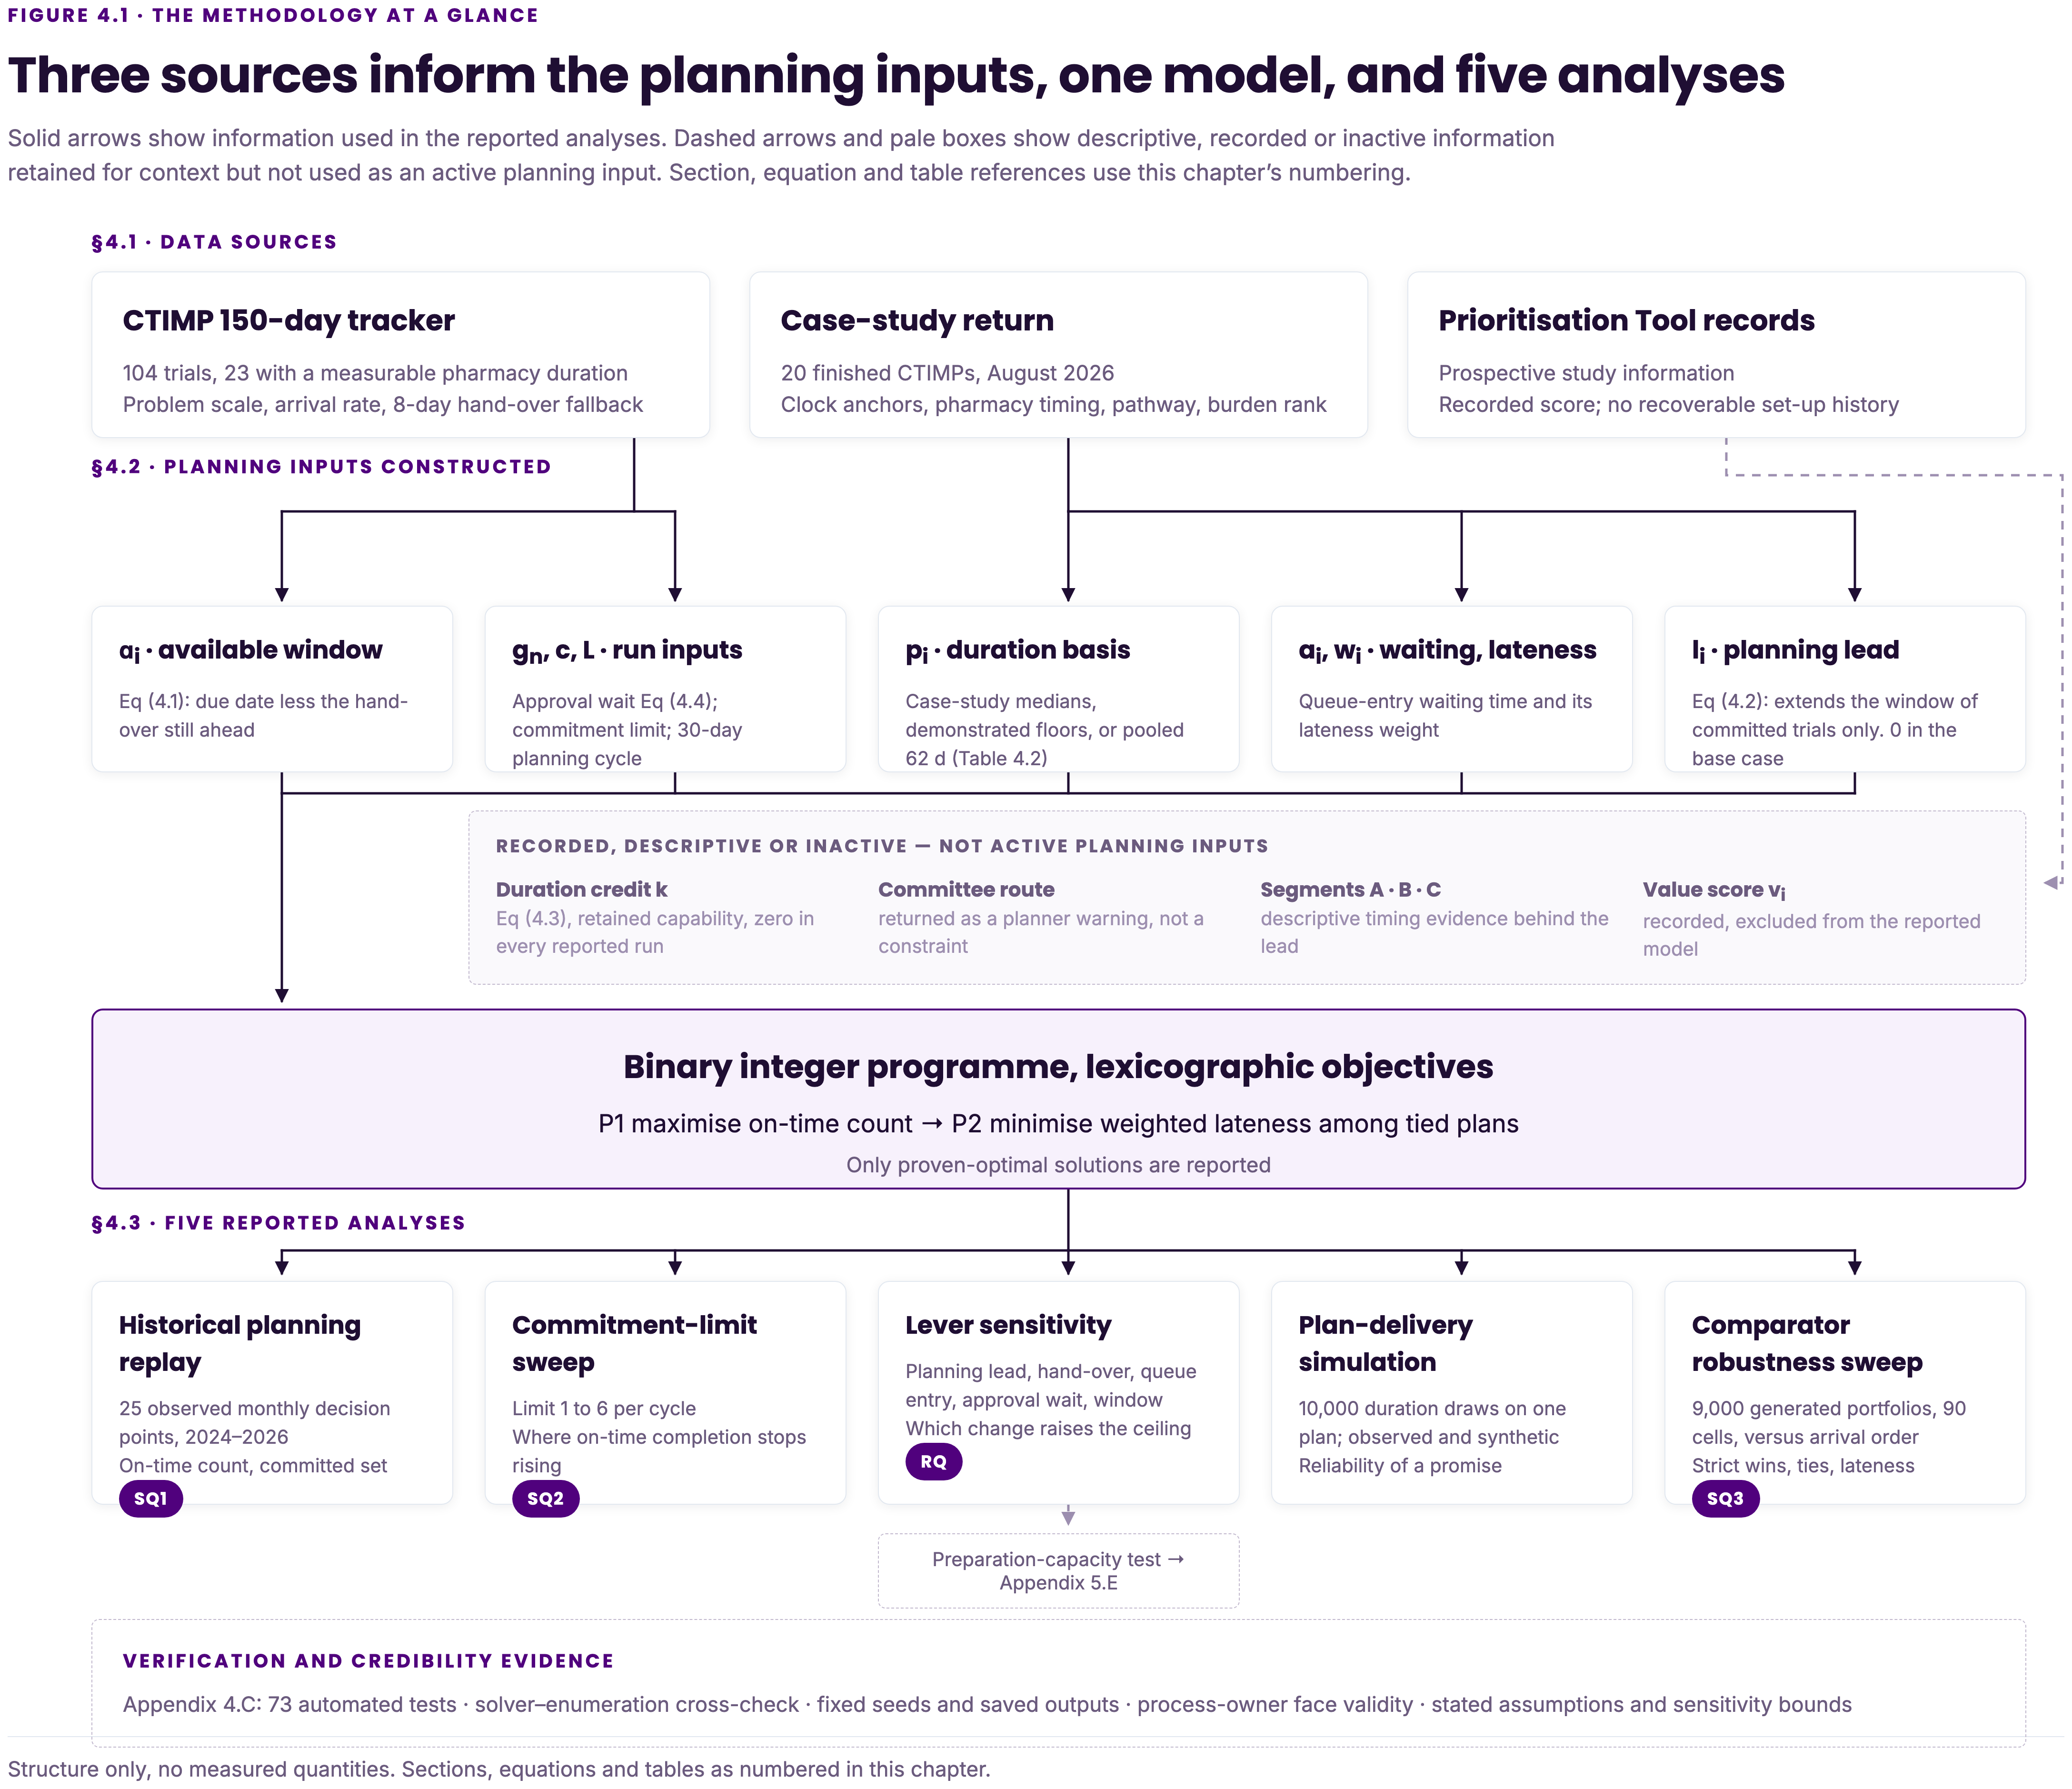
\includegraphics[width=\textwidth]{fig4_1_methodology_map.png}
  \caption{From operational records to research-question evidence}
  \label{fig:datasources}
\end{figure}

\section{Constructing the planning inputs}
\label{sec:parameters}

Four quantities decide a plan. Appendix 4.J tabulates every parameter, its source, and the two quantities deliberately excluded.

\subsection{Days available, which is not days remaining}
\label{sec:available}

A trial's available time is the period from the point at which pharmacy can begin work to its due date:

\begin{equation}
  \alpha_i = due_i - \max(\text{today}, \; \text{queue entry}_i)
  \label{eq:available}
\end{equation}

The calculation subtracts hand-over delay that is still ahead of the trial, but not delay already served. This distinguishes the nominal 60-day deadline from the time pharmacy can actually use; Figure~\ref{fig:segments} illustrates the distinction.

\begin{figure}[htbp]
  \centering
  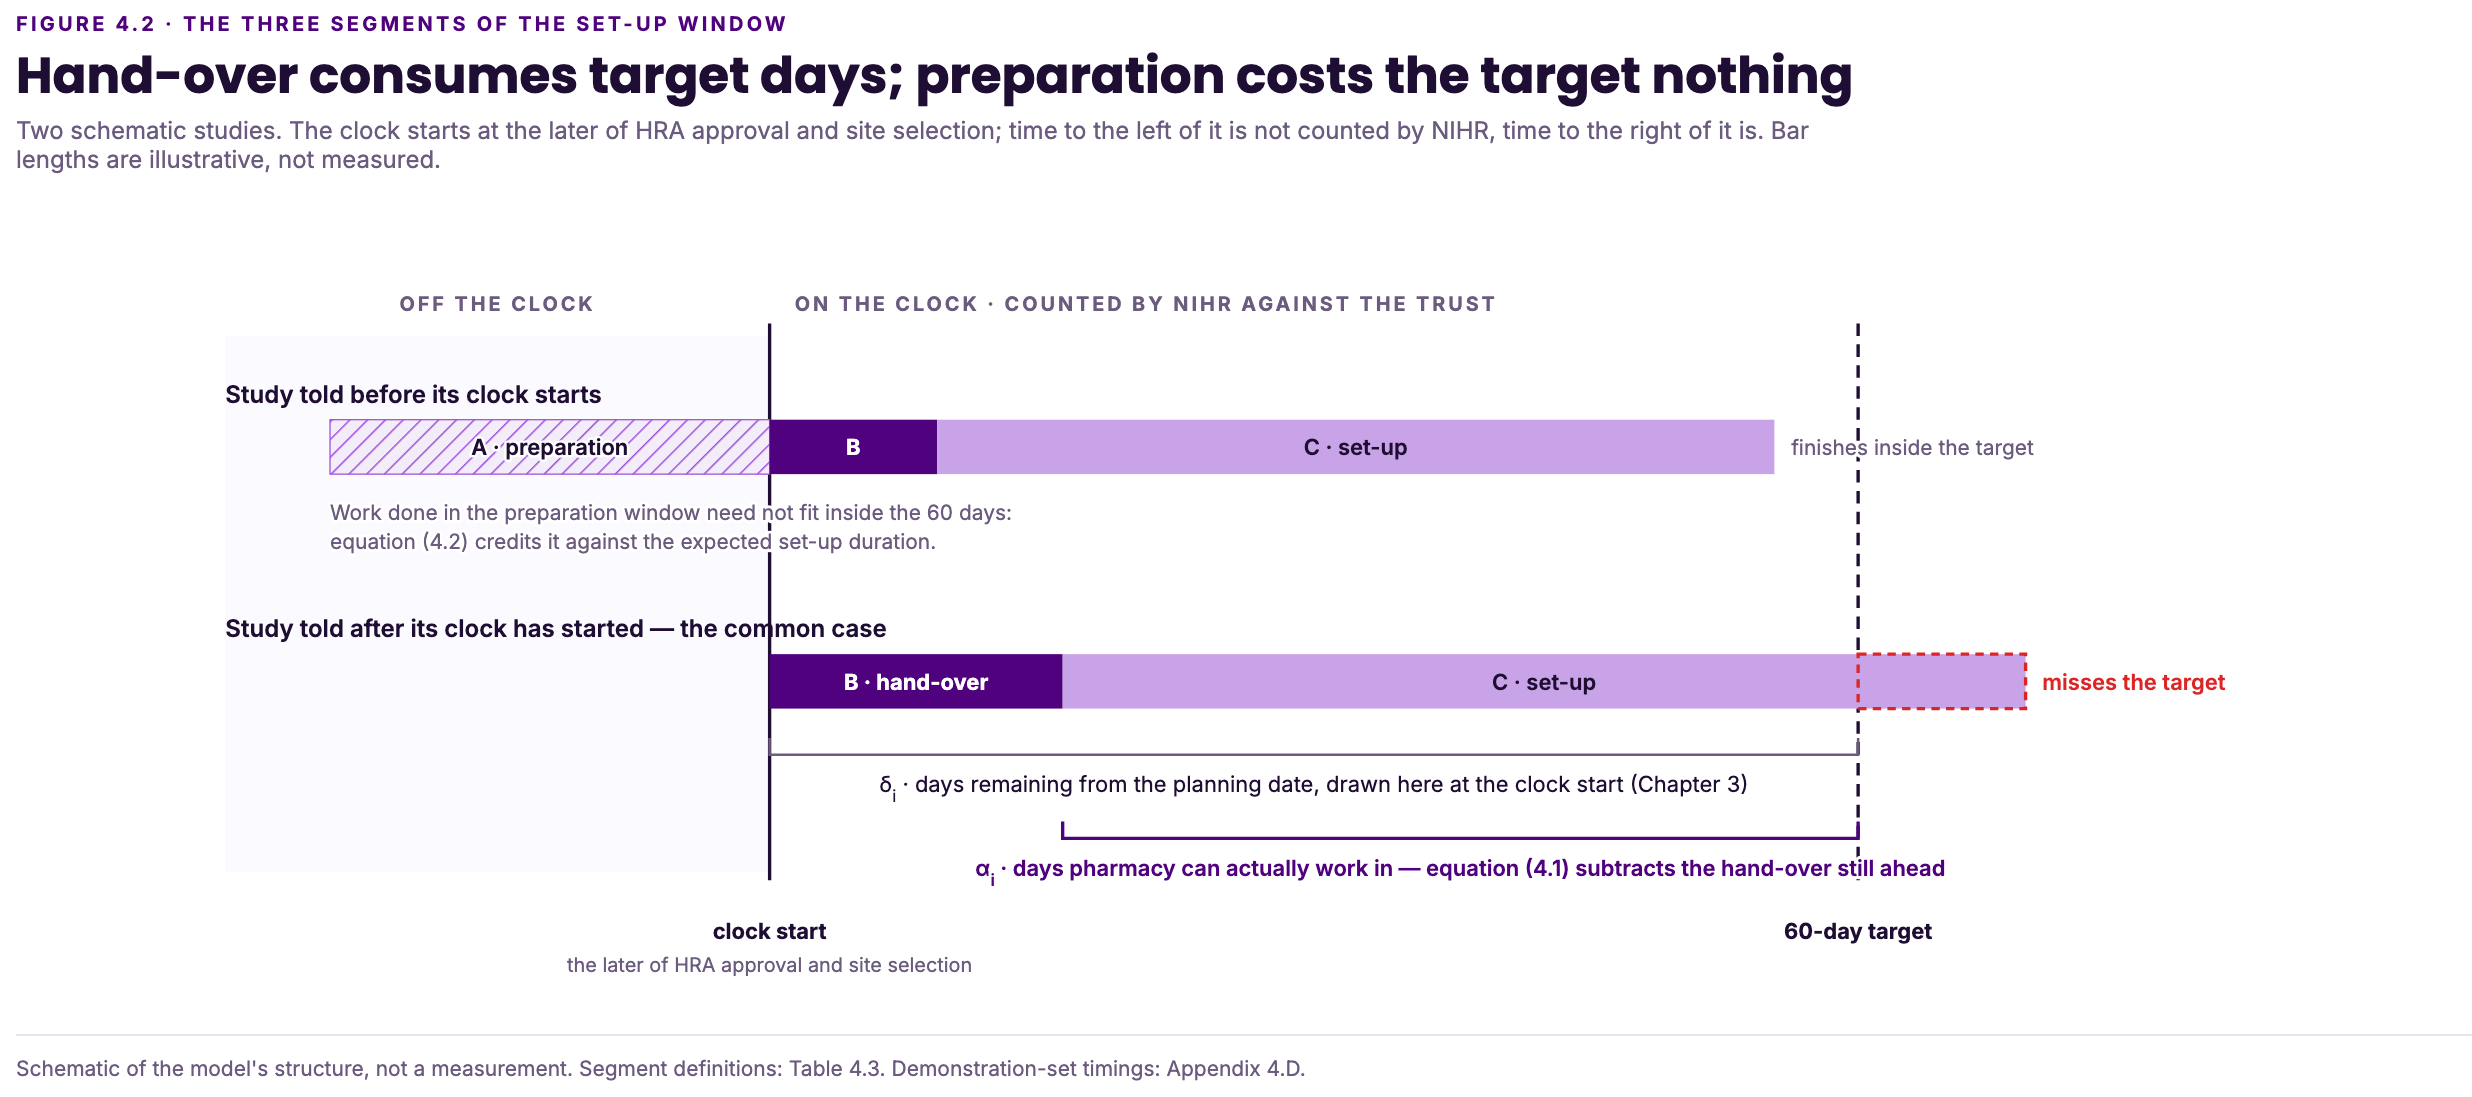
\includegraphics[width=\textwidth]{fig4_2_segment_schematic.png}
  \caption{Hand-over consumes target days; preparation costs the target nothing \emph{Note.} A schematic of the model's structure, not a measurement. Measured distributions are in Appendix 4.D.}
  \label{fig:segments}
\end{figure}

\subsection{Set-up duration, treated as uncertain}
\label{sec:casestudies}

The duration basis differs by analysis. Current-performance regimes use elapsed case-study durations, whereas the demonstrated planning floors are derived from recorded work intervals. All duration measures end at pharmacy green light, but their start events differ; Appendix 4.H defines each interval and Appendix 4.B considers the resulting overlap with approval delay. Across the 19 usable work intervals, the median was 79 days, with a range of 23 to 262 days; five fitted within the 60-day target.

\begin{table}[htbp]
  \centering
  \caption{The five duration regimes}
  \label{tab:regimes}
  \begin{tabularx}{\textwidth}{@{}lLL@{}}
    \toprule
    \textbf{Regime} & \textbf{What it represents} & \textbf{Where used} \\
    \midrule
    0.8 times the case-study medians & Current performance 20\% faster & Appendix 5.A \\
    \addlinespace
    1.0 times the case-study medians & Current performance & Appendix 5.A \\
    \addlinespace
    1.2 times the case-study medians & Current performance 20\% slower & Appendix 5.A \\
    \addlinespace
    The demonstrated work floors & Routine 50; Prescription-only 30; Aseptic-only 72; Both 60 days. A 63-day overlay applies only to high-burden studies on the Both pathway & §Section~\ref{sec:realqueues} to 5.6, Appendix 5.A \\
    \addlinespace
    The pooled first-quartile figure of 62 days & One achievable benchmark across pathways & Appendix 5.A \\
    \bottomrule
  \end{tabularx}
\end{table}

High burden means a rank of 5 or 6 on the scale pharmacy returned; Appendix 4.H distinguishes the burden-band minima, the pathway floors and the 63-day overlay, and Appendix 4.F explains why that rank is the one used.

The floors are demonstrated-achievable standards rather than forecasts or raw minima; Appendix 4.H derives and audits them. Results computed on them describe an optimistic operating condition rather than an expected one.

\subsection{Preparation and approval}
\label{sec:preparation}

Preparation does not shorten the total work a trial requires; it moves part of that work outside the target window. The case studies suggest that earlier starts change how much work falls within the target window rather than the observed work duration itself: work intervals did not differ detectably between early and late starters, whereas on-time outcomes did (Appendix 4.I).

The reported preparation analysis represents an earlier planning lead, which for committed trials increases the time available before the 60-day deadline. It is interpreted operationally as work that can begin before the target clock starts, rather than as evidence that underlying set-up duration is shorter. Writing $\ell_i$ for the lead assigned to a committed trial:

\begin{equation}
  \alpha_i^{\text{lead}} = \alpha_i + \ell_i
  \label{eq:lead}
\end{equation}

The lead is granted only to committed trials and is zero in the base case; Appendix 4.J.3 gives the implementation.

The base analysis does not charge pre-window preparation against the cycle commitment limit. This isolates the time benefit of earlier preparation from its operational resource cost; Appendix 5.E tests the sensitivity of that simplification by reducing the concurrent capacity available to the plan.

The implementation retains a separate duration-credit capability, but it is inactive in every reported analysis and produces no Chapter 5 result; its specification and verification are retained in Appendix 4.J.4 and Appendix 4.C, Tests 24 to 35.

Final approval is a shared, load-dependent queue. The wait $g_n$ uses the Pollaczek-Khinchine formula for a single server, exact when its assumptions hold and needing only the mean and variability of approval time, not its shape, which this study cannot observe:

\begin{equation}
  g_n = \frac{\rho}{1-\rho} \cdot \frac{1+\kappa^2}{2} \cdot s, \qquad \rho = \min\left(0.95,\; \frac{n\,s}{A}\right)
  \label{eq:pk}
\end{equation}

Approval time is unobserved and is therefore treated as a sensitivity parameter; Appendix 4.B records the queueing assumptions, the utilisation and variability values, and the overlap analysis.

\section{Experimental design}
\label{sec:experiments}

Every run builds a plan by the process in Figure~\ref{fig:solution}, differing only in what it varies before that process starts and records after it ends. The model maximises on-time completions first and then minimises weighted lateness among tied plans. For Section~\ref{sec:tradeoff}, the model also reports the least-late plan at each achievable on-time count to display the trade-off; these are count-constrained comparisons, not alternative lexicographic optima. Appendix 4.J provides the formulation and solver settings.

\begin{figure}[htbp]
  \centering
  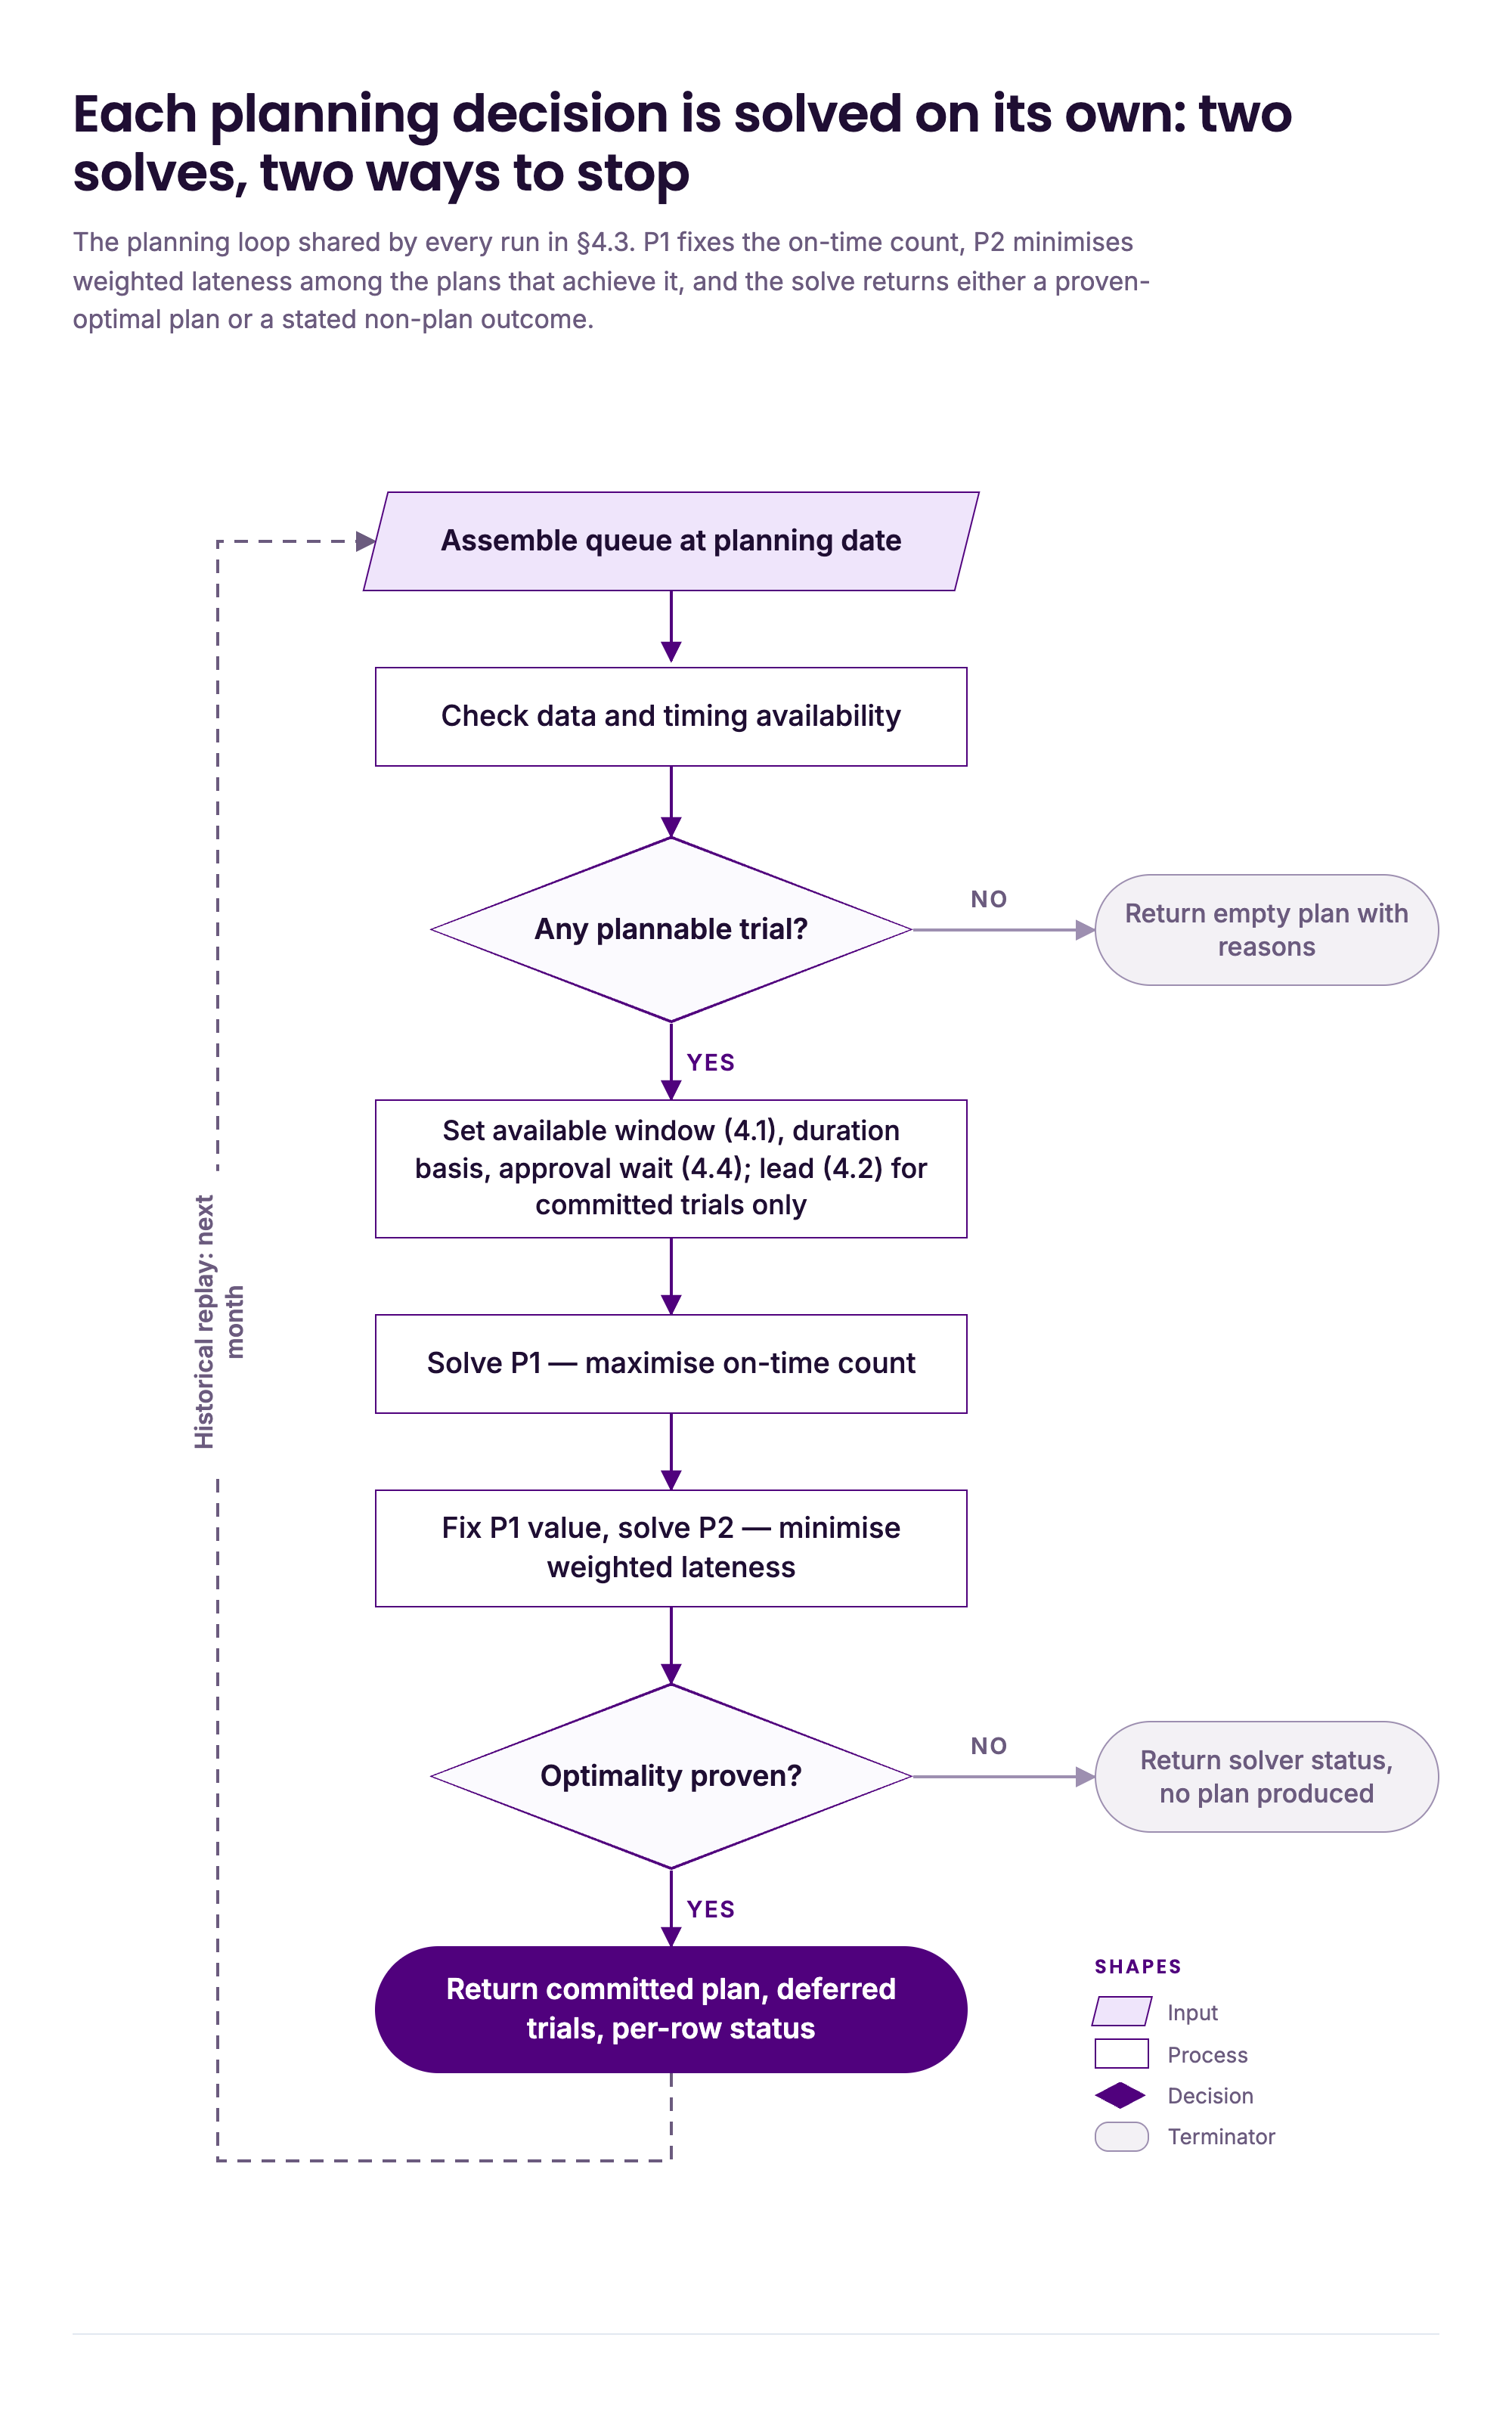
\includegraphics[width=\textwidth]{fig4_3_solution_construction.png}
  \caption{Solution construction process \emph{Note.} The dashed return arrow applies to the historical replay only: each month is solved independently and no slot is held open for a later one.}
  \label{fig:solution}
\end{figure}

\begin{table}[htbp]
  \centering
  \caption{Analysis-to-question map}
  \label{tab:analyses}
  \begin{tabularx}{\textwidth}{@{}lLLLL@{}}
    \toprule
    \textbf{Analysis} & \textbf{Data basis} & \textbf{What varies} & \textbf{What it measures} & \textbf{Question} \\
    \midrule
    Historical planning replay & Observed queues & 25 monthly decision points, 2024 to 2026 & On-time trials, committed set & SQ1 \\
    \addlinespace
    Commitment-limit sweep & Observed queues & Commitments per cycle, 1 to 6 & Whether raising the commitment limit changes on-time completion or weighted lateness & SQ2 \\
    \addlinespace
    Lever sensitivity & Observed queues & Preparation, hand-over, queue entry, approval, target window & Which change raises the ceiling & RQ, SQ2 \\
    \addlinespace
    Plan-delivery simulation & Observed and synthetic queues & 10,000 duration draws on one plan & Reliability of a promised outcome & RQ \\
    \addlinespace
    Comparator robustness sweep & Generated portfolios & 9,000 portfolios, 90 scenario cells & Strict wins over arrival order, and their cost & SQ3 \\
    \addlinespace
    Targeted-preparation comparison & Observed queues & Lead to high-burden committed trials only, against all committed trials & On-time coverage and the early-notification days required & Appendix 5.B \\
    \addlinespace
    Preparation-capacity test & Observed queues & Preparation lead against reduced capacity & Whether the preparation finding survives & Appendix 5.E \\
    \bottomrule
  \end{tabularx}
\end{table}

Nineteen case studies enter the replay, being those with both clock anchors; BALLOON has no site-selected date and BRISOTE no recorded start. Appendix 4.J holds the run settings, of which one hands-on day per approval is the only input in Chapter 5 not measured.

Two simulations are reported separately. The plan-delivery simulation tests the reliability of a selected plan under duration uncertainty, whereas the robustness sweep tests whether the selection rule outperforms arrival order across generated portfolios. Appendix 4.J specifies their distributions, settings and reporting rules.

\subsection{The comparator and the robustness sweep}
\label{sec:comparison}

\textbf{The comparator is arrival order} (Section~\ref{sec:inpractice}): it commits the longest-waiting eligible trials up to the same commitment limit as the model. Both plans run through Figure~\ref{fig:solution} under identical windows, duration assumptions and approval waits, so any difference arises from the selected set alone. Because practice may informally expedite some studies, the comparator result is an upper bound on the model's advantage over routine practice.

The sweep generates portfolios that vary arrival timing, pathway composition and duration regime, and reports the count in which the model places strictly more trials inside the window, with ties and the weighted-lateness difference beside it. Appendix 4.J.6.1 specifies the design and states why ties are read at cell level rather than pooled. \textbf{Table 5.A.2 summarises the sweep by duration regime and is the principal test of SQ3}; Appendix 5.A holds the grid.

\section{Credibility, assumptions and boundaries}
\label{sec:verification}

\textbf{Verification, reproducibility and face validity.} Automated tests verify input construction, optimisation logic, simulation behaviour and agreement between enumerated and solver solutions, with the full inventory in Appendix 4.C. All simulation runs use fixed seeds and save dated outputs, so Chapter 5 figures can be regenerated exactly. R\&I and pharmacy reviewed the process representation and input definitions, which constitutes face validity from process owners rather than independent validation.

\textbf{A known overlap, bounded rather than removed.} Each planning duration ends at the pharmacy green light, which is the approving signature, so it already includes part of the wait that equation~(\ref{eq:pk}) adds separately. That component is dated in no system and cannot be separated, so the overlap is retained as a bounded conservative approximation rather than an empirically identified separation of work and approval delay; Appendix 4.B gives the assumption audit and the sensitivity result.

\textbf{What the evidence cannot establish.} Three limits bound every result. Set-up start dates are estimates, so the durations of Section~\ref{sec:casestudies} carry recall error the data cannot quantify. Hands-on approval time is unmeasured, so the checks above verify the implementation and not the formulation behind equation~(\ref{eq:pk}); testing that needs a separate model of the approval-signature queue, recorded as future work in Chapter 6. And the generated data of Section~\ref{sec:experiments} answer questions the observed queues cannot, but do not evidence the trust's own portfolio. All three are handled by stated assumption, sensitivity analysis and simulation rather than presented as observed fact.

---


% Chapter 5, Results.
% Generated from Dissertation/Chapter5_Results.md by tools/md2tex.py.
%% The draft-status line, the provenance notes and the [edit] markers in the
%% Markdown source are not part of the submitted text and are absent here.
%% Markdown is the source. Regenerate this file when it changes; do not hand-edit.

\chapter{Results}
\label{ch:results}
\lhead{Chapter 5. \emph{Results}}

This chapter reports what the planning model returns on the trust's own queues. It gives the capacity ceiling and which trials reach it, tests how reliably a plan delivers what it promises, and identifies what limits the number and what raising it costs. Table~\ref{tab:analyses} maps each analysis to the sub-question it answers.

\section{The model's decision on the real queues}
\label{sec:realqueues}

The model was solved at each of the 25 decision points of Section~\ref{sec:experiments}. Figure~\ref{fig:planactual} sets its plan against what the service actually did.

\begin{figure}[htbp]
  \centering
  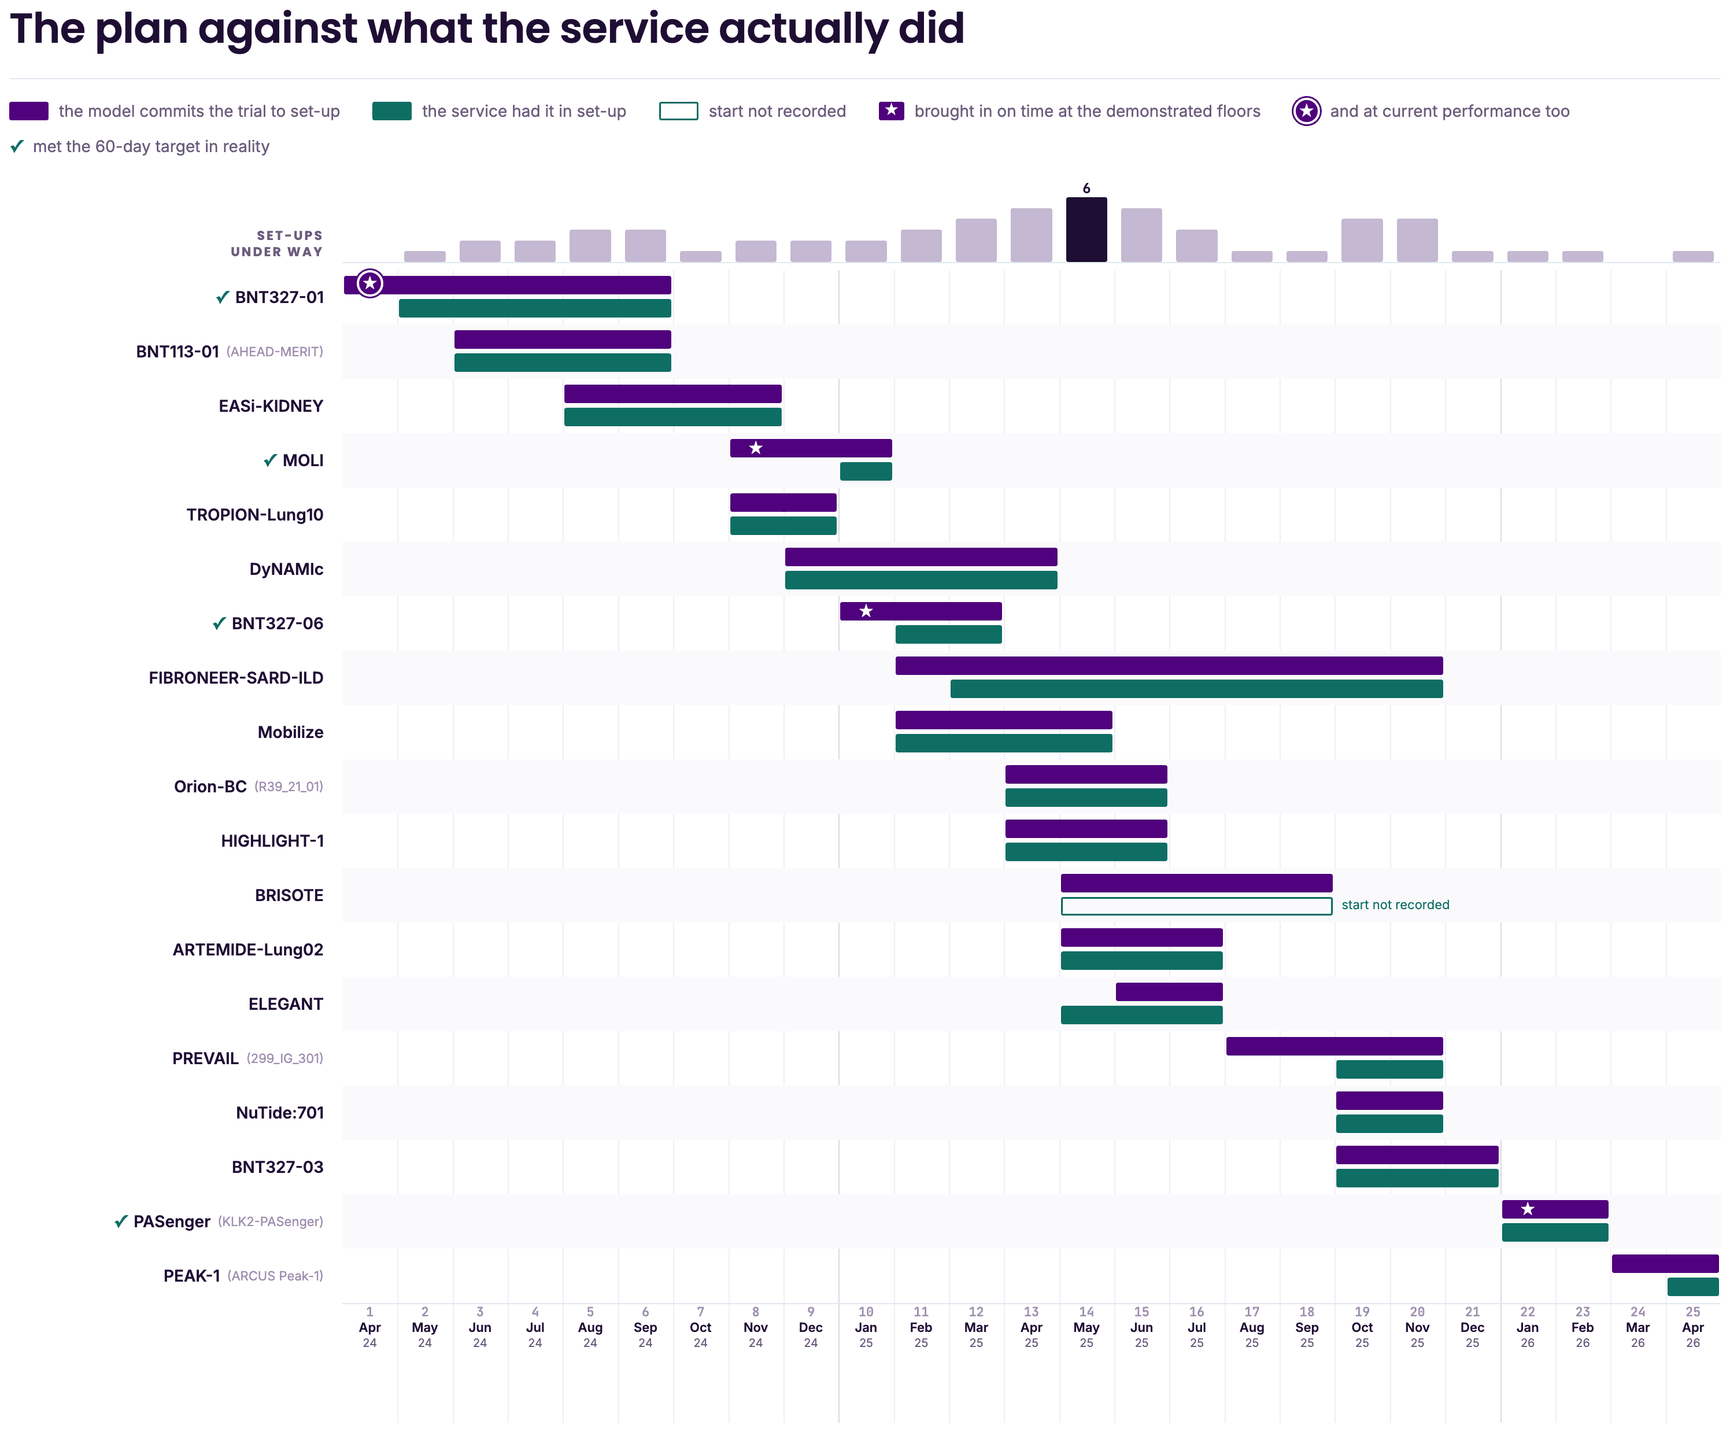
\includegraphics[width=\textwidth]{fig5_1_plan_vs_actual.png}
  \caption{The plan against what the service actually did, by month of commitment rather than by date}
  \label{fig:planactual}
\end{figure}

Only four trials ever finish on time, and they are exactly the four that met the target in reality. The model identifies these trials in advance rather than in hindsight; it does not uncover any additional trial that the service could have brought in on time.

Against the stated ``commit the longest waiter'' rule, the model performs better when capacity is limited. It brings a trial in on time in 10 of the 25 months at both one and two set-ups per month, compared with 6 and 7 months respectively for the rule. From three set-ups per month onwards, both approaches commit the same trials and perform equally.

The 10 months cover only four trials. Because the plan is remade each month, a trial that still fits is re-committed and counted again. The comparator is a stated arrival-order rule, not an observed record of practice.

A sweep of 9,000 synthetic portfolios tests whether that pattern holds beyond the trust's own queues. At current performance the model never beats the arrival-order rule for on-time completions. At the demonstrated floors it wins in 36\% of cases, each win costing 24.3 weighted days of lateness elsewhere, and it helps most when trials arrive early and the aseptic share is low. Appendix 5.A holds the design, the limitations and the full grid.

\section{Why the model picks these and not others}
\label{sec:whythese}

The model starts the right trials sooner. Three of the four trials it brings in on time are among the six it starts earliest: MOLI by 34 days, BNT327-06 by 22 days, and BNT327-01 by 17 days. Appendix 5.D sets the model's start date against the service's own for all nineteen.

The service's own head start bought little: of the twelve trials it began before the model would, eleven missed the target anyway. Waiting is what consumes the window, and the trial that can still finish is usually the one that has just arrived; Appendix 5.D works through November 2024.

Figure~\ref{fig:allcases} shows why so few can finish at all, placing the 19 studies with a computable clock start on one axis measured in days from that start.

\begin{figure}[htbp]
  \centering
  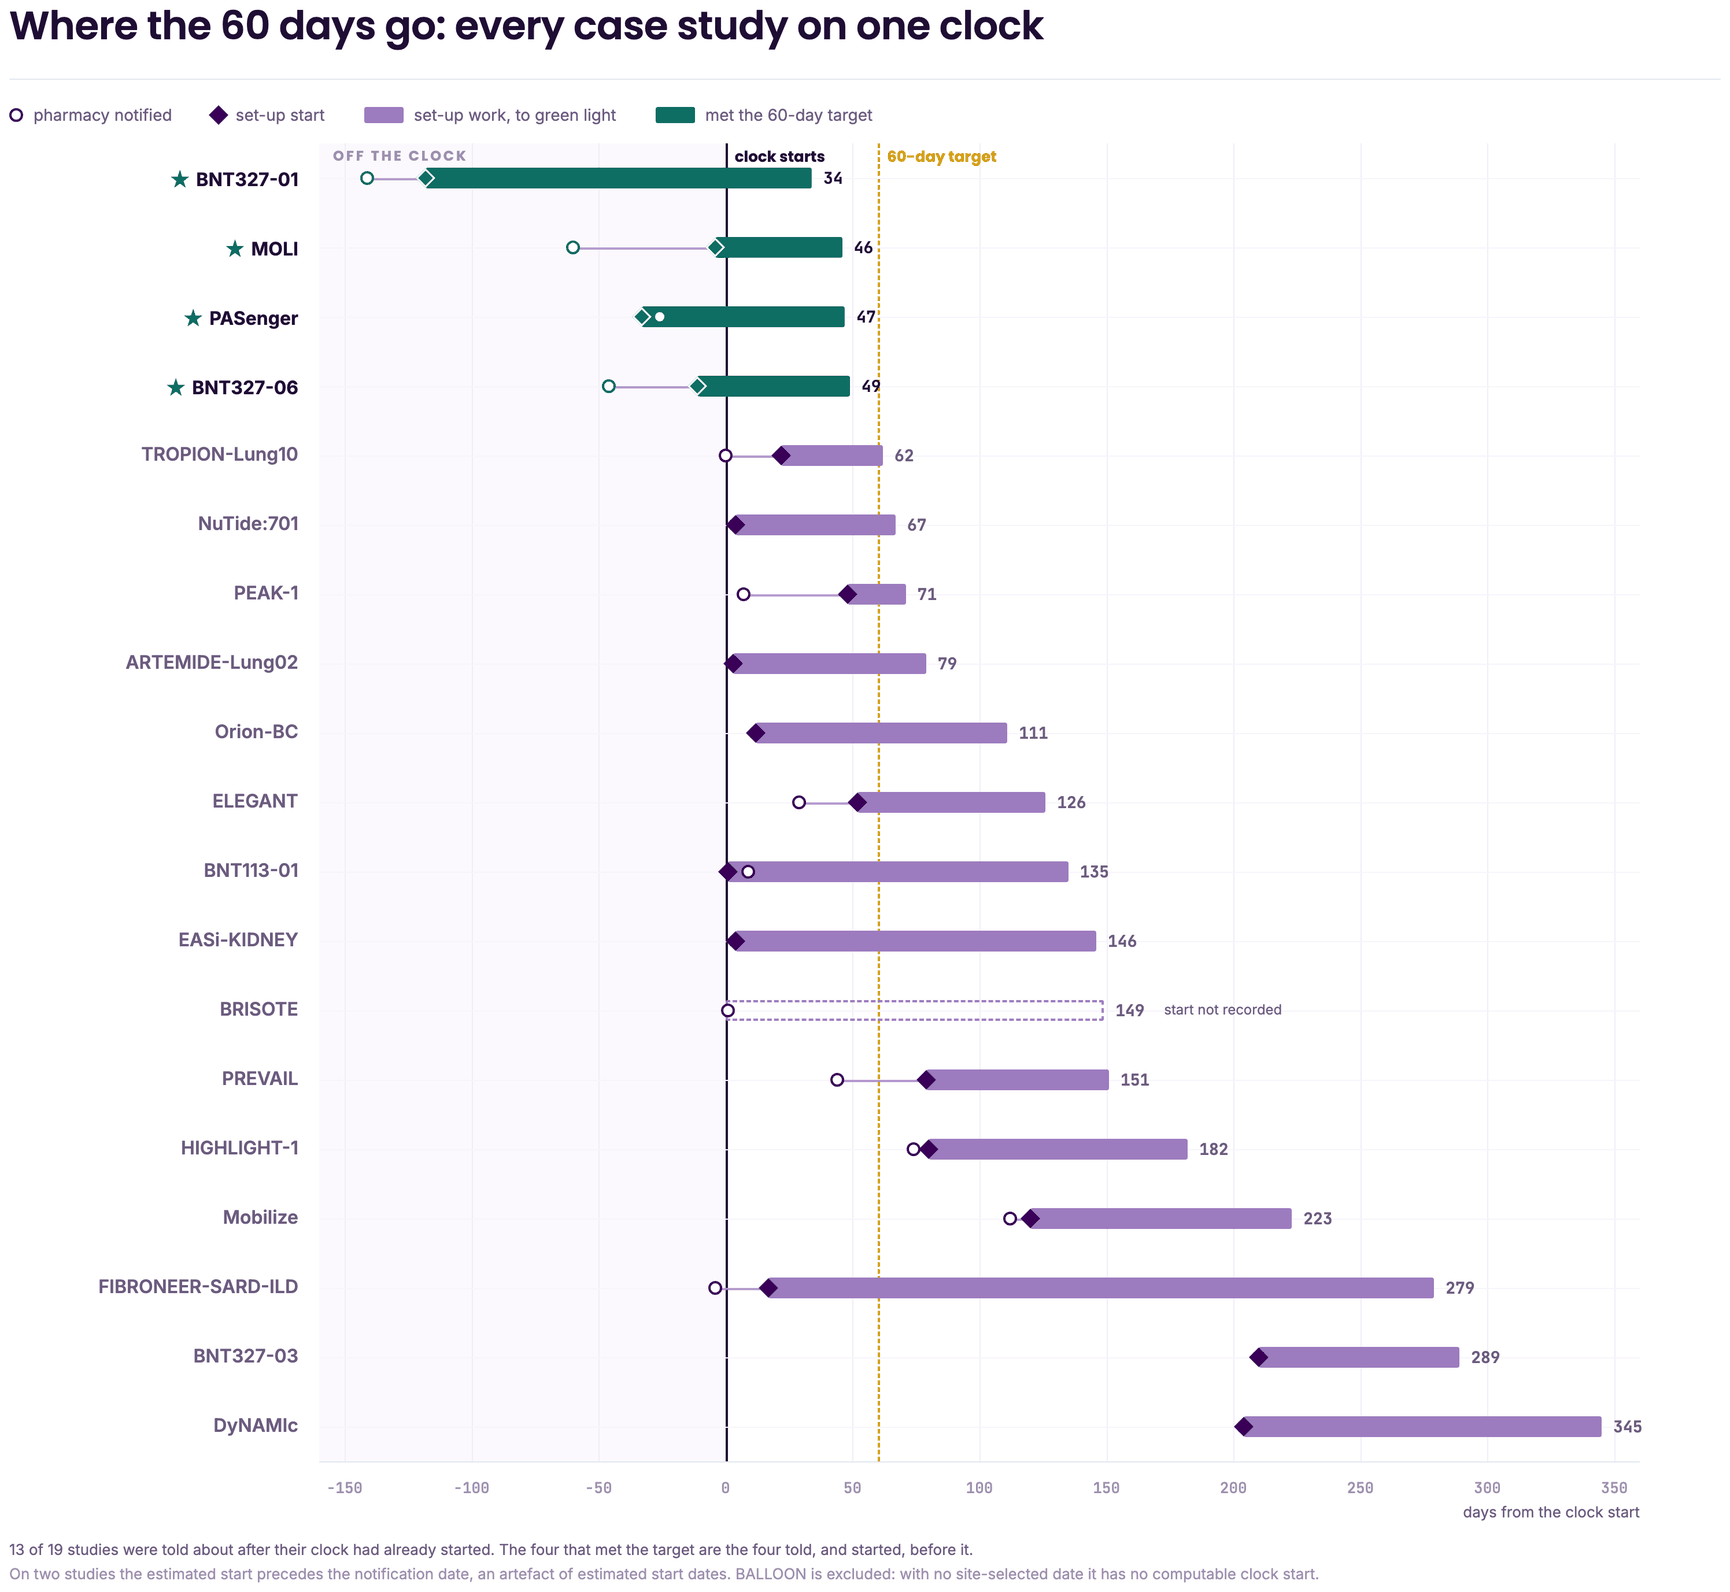
\includegraphics[width=\textwidth]{fig5_3_all_cases_timeline.png}
  \caption{Where the 60 days go: every case study on one clock}
  \label{fig:allcases}
\end{figure}

Four trials met the target, and all entered the pharmacy queue before the 60-day clock began.

\begin{table}[htbp]
  \centering
  \caption{The four trials that met the 60-day target}
  \label{tab:fourtrials5}
  \begin{tabularx}{\textwidth}{@{}lLLL@{}}
    \toprule
    \textbf{Trial} & \textbf{Days entered before clock start} & \textbf{Work interval (days)} & \textbf{Clock interval (days)} \\
    \midrule
    MOLI & 4 & 50 & 46 \\
    \addlinespace
    BNT327-06 & 11 & 60 & 49 \\
    \addlinespace
    PASenger & 33 & 80 & 47 \\
    \addlinespace
    BNT327-01 & 118 & 152 & 34 \\
    \bottomrule
  \end{tabularx}
\end{table}

Starting earlier did not shorten the work. Work intervals did not differ significantly between early and late starters ($p = 0.71$). Instead, earlier starts moved some work outside the 60-day window. Two of the four trials met the target despite requiring more than 60 days of work because their set-up began before the window opened. The window did not stretch; the work began earlier. No recorded trial characteristic predicted an early start (Appendix 4.I).

Where the plan falls short, it does so by relatively little. Four trials missed the target by 20 days or less in reality and, under the plan, fall 10 to 29 days short of their available windows. This shortfall reflects insufficient time in the window, not a failure to choose between trials. No selection rule can recover those days; Section 5.4 examines what would add them.

\section{Plan delivery under duration uncertainty}
\label{sec:delivery}

A solved plan produces one on-time count from a single planned duration for each pathway, so the uncertainty run of Section~\ref{sec:experiments} and Appendix 4.J.6.2 replays each committed plan 10,000 times to report how often that count is actually met. Appendix 5.F reports what the real February queue delivers, and Figure~\ref{fig:planuncertainty} the synthetic one.

In the real February queue, neither duration basis produced a plan promising an on-time completion. The simulation therefore describes outcome variability rather than delivery reliability for a positive promise; approval delay is held at its expected value throughout, so every reported figure understates total uncertainty. Appendix 5.F reports the distribution.

The synthetic standing queue of 16 trials described in Appendix 4.G, used in this section alone and labelled synthetic throughout, is the one that carries a promise. At current performance it promises zero and delivers zero in every one of the 10,000 runs. At the demonstrated floors it promises three, and Figure~\ref{fig:planuncertainty} shows what arrives: three in 32.6\% of runs, but two in 48.5\%. The promised three therefore lands in about a third of runs, two is the most likely single outcome, and one is the highest count reached in at least 90\% of runs.

\begin{figure}[htbp]
  \centering
  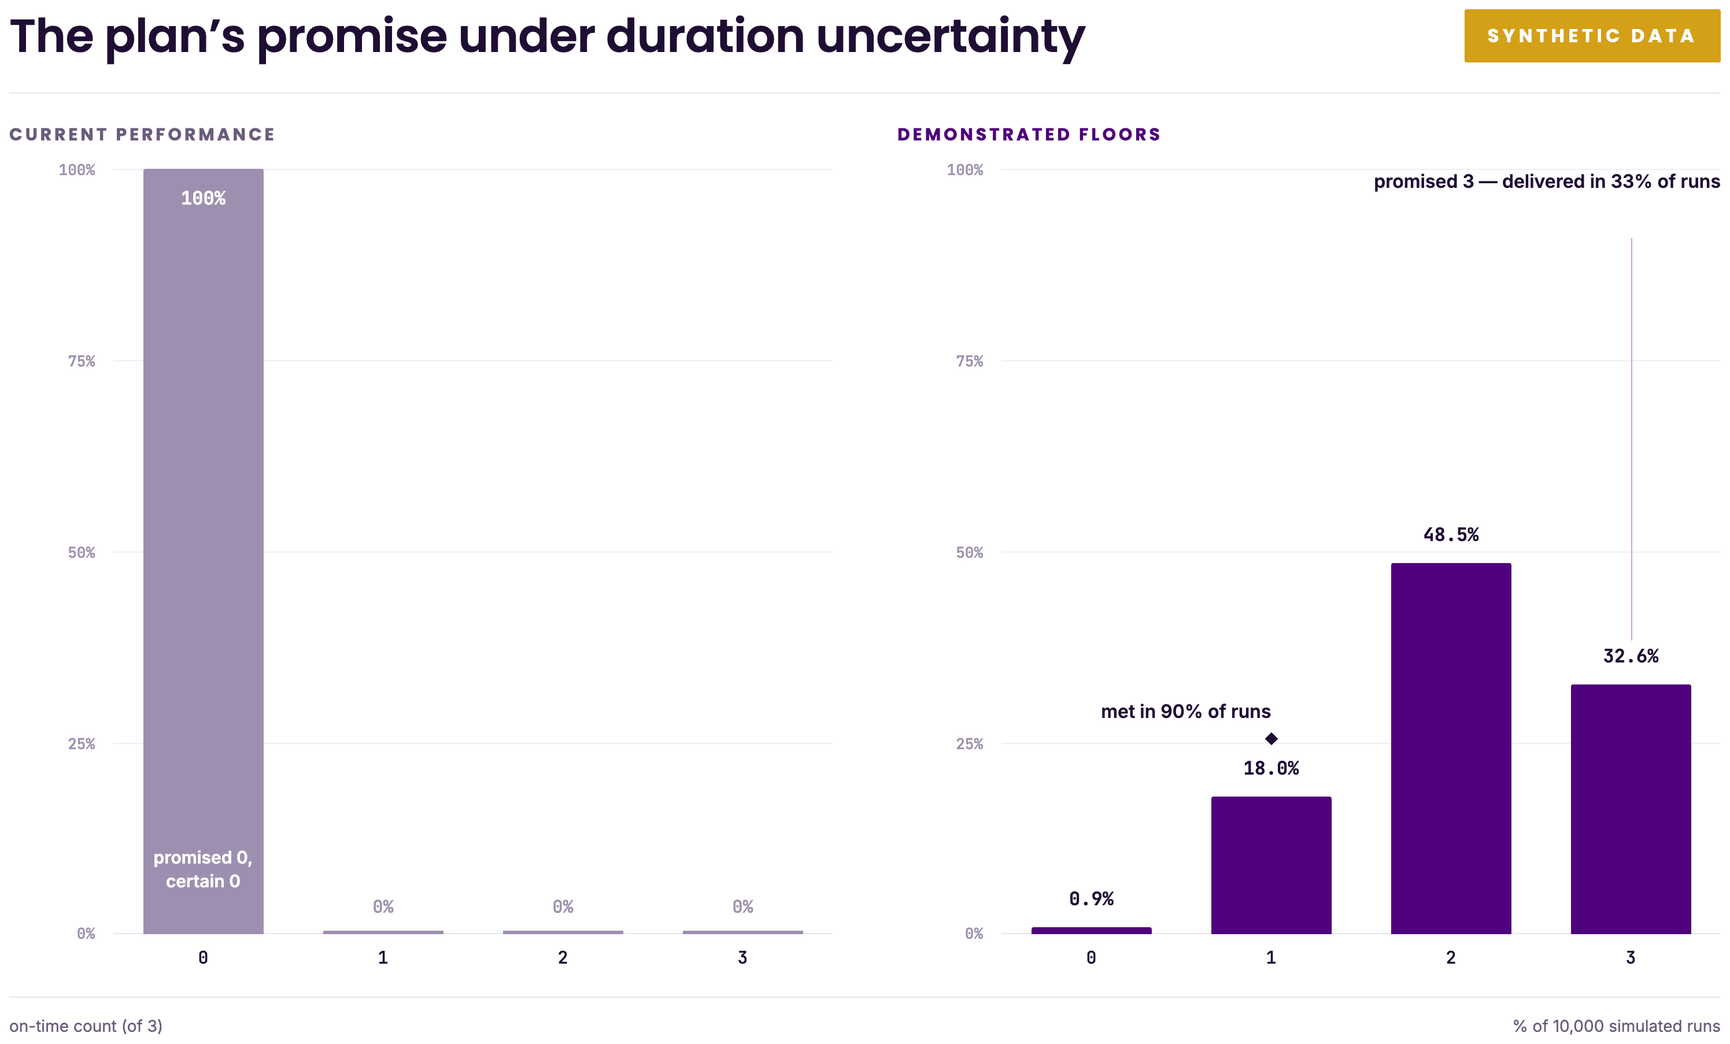
\includegraphics[width=\textwidth]{fig5_4_plan_uncertainty.png}
  \caption{The plan's promise under duration uncertainty (synthetic queue)}
  \label{fig:planuncertainty}
\end{figure}

The point is the deterministic verdict, not any single trial. Where a plan records a trial as one day late, that margin sits well inside the observed spread of set-up durations, so the label carries no information and a trivial change of input reverses it. Where the margin is smaller than the spread, the deterministic result is a tie-break rather than a finding; Appendix 5.F works through the case behind this.

\section{What would have to change}
\label{sec:levers}

Six settings could change the results. Table~\ref{tab:settings} reports what each one does, and the two columns disagree in a way that matters.

\begin{table}[htbp]
  \centering
  \caption{What each setting changes, across twenty-five decision points}
  \label{tab:settings}
  \begin{tabularx}{\textwidth}{@{}lLLLL@{}}
    \toprule
    \textbf{Setting} & \textbf{Intervention tested / observed span} & \textbf{Months $\geq$1 on time (of 25)} & \textbf{Best count} & \textbf{Largest single-date lateness reduction} \\
    \midrule
    Preparation lead, committed trials & 0, 7, 14, 21, 35, 60 days & 20 of 25 & 3 & 394 \\
    \addlinespace
    Pharmacy queue, notification to start & Return 0, 25, 50, 75 or 100\% of each trial's observed wait, which spans 0 to 23 days & 14 of 25 & 2 & 76 \\
    \addlinespace
    Hand-over gap, clock to notification & Return 0, 25, 50, 75 or 100\% of each trial's observed gap, which spans 0 to 112 days & 11 of 25 & 2 & 498 \\
    \addlinespace
    Slots opened per month & 1, 2, 3, 4, 5, 6 & 9 of 25 & 1 & 154 \\
    \addlinespace
    Hands-on days per approval & 0.5, 1.0, 2.0, 3.0 days & 9 of 25 & 1 & 20 \\
    \addlinespace
    Target window & 55, 60, 65, 70 days & 11 of 25 & 2 & 77 \\
    \bottomrule
  \end{tabularx}
\end{table}

\noindent\footnotesize Note. R\&I controls the preparation lead and the hand-over gap, pharmacy the queue and the slots, the approver the hands-on days and governance the target window; every lever is measured except hands-on days, which is assumed, and the target window, which is policy. For the two delay levers the percentages apply to each trial's own observed delay, so the day spans are observed across trials rather than common tested values. The final column is the largest single-date reduction in weighted lateness against that lever's baseline, not a total. Appendix 4.J.7 gives the full design.\normalsize

Nine of the twenty-five dates already admit one on-time trial at the demonstrated floors under the high-burden overlay and with no further change, which is the row every other row must be read against.

The levers affect the two outcomes differently. Removing the hand-over gap produces the largest reduction in weighted lateness but few additional on-time trials, because many affected cases are already beyond rescue. Reducing the pharmacy queue removes less lateness but creates more on-time completions by affecting trials near the threshold. Appendix 5.C gives the values.

Apart from preparation, no setting reaches three on-time trials in any month: the two delays and the target window reach two, and slots and approval time never pass one. Everything except preparation therefore moves more months onto the target without raising the ceiling. Appendix 5.C draws four of them as surfaces.

Preparation is the only setting that creates this opportunity, and Figure~\ref{fig:preparation} shows its effect on the portfolio. Appendix 5.E tests the capacity assumption of Section~\ref{sec:preparation} by reducing the concurrent capacity available to the plan.

\begin{figure}[htbp]
  \centering
  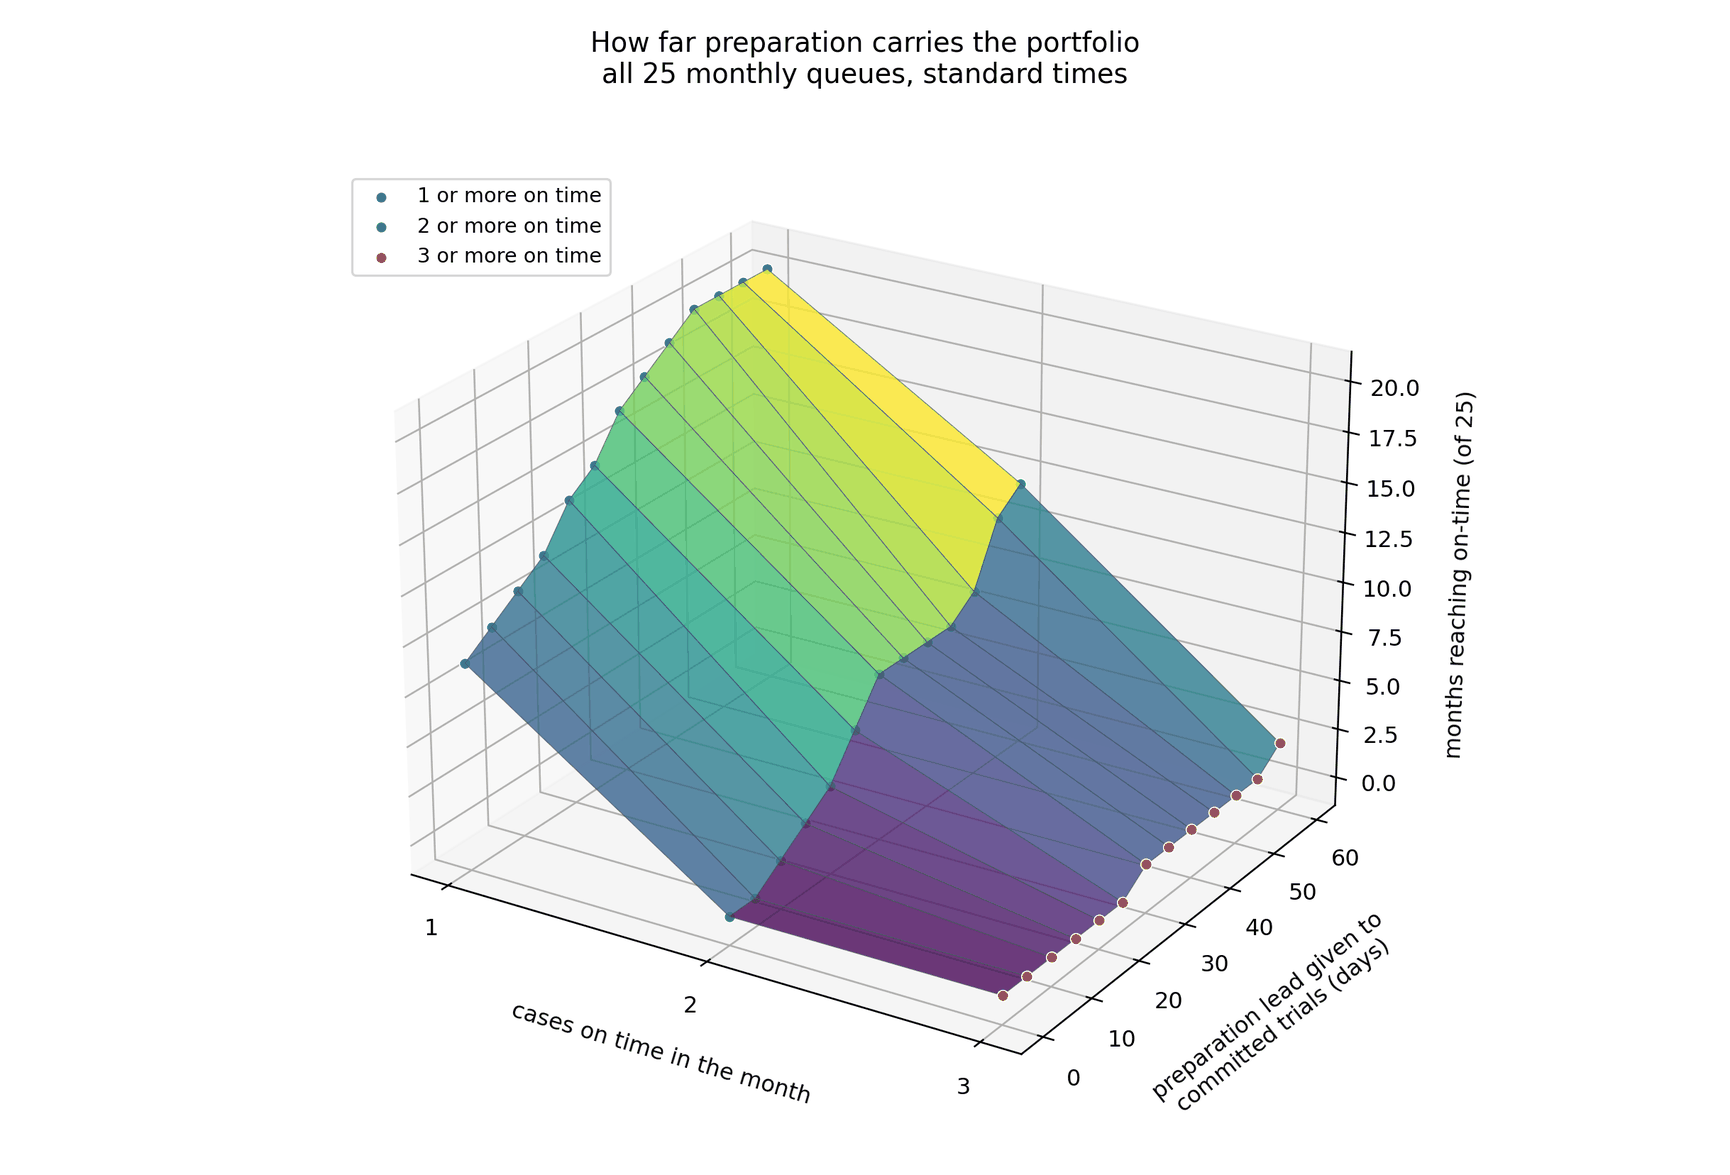
\includegraphics[width=\textwidth]{fig5_7_preparation_surface.png}
  \caption{How far preparation carries the portfolio}
  \label{fig:preparation}
\end{figure}

Approval time is the only assumption in the table without direct measurement, because the August 2026 questionnaire gave a range rather than a value. The commitment limit is a maximum, not a requirement: if opening six set-ups would create a long signature queue, the model commits fewer trials instead. Approval time therefore limits how much capacity is usable, not the on-time ceiling. Appendix 5.C reports the wait at each level and how many set-ups are worth opening.

\section{Which studies preparation should reach}
\label{sec:targeting}

Table~\ref{tab:settings} makes preparation the strongest lever; pharmacy burden says which studies should receive it.

Burden does not make set-up take longer: the work-duration distributions for the three burden bands do not differ significantly (Kruskal-Wallis $p = 0.557$). Instead, burden raises the fastest observed duration in each band: 23 days for low burden, 40 for medium burden, and 60 for high burden (Table 4.H.3). This leaves 37 days of slack within the 60-day target for low-burden trials, 20 for medium-burden trials, and none for high-burden trials.

The median time between the target clock starting and pharmacy receiving the study is 14 days (Appendix 4.D); low- and medium-burden trials can absorb this delay. High-burden trials cannot absorb even one day; Figure~\ref{fig:burdenslack} sets the three bands against the window. The exclusion is therefore structural. Of the six high-burden trials, the two that began before the clock started met the target, whereas all four that began afterwards missed it (Fisher's exact test, $p = 0.067$).

\begin{figure}[htbp]
  \centering
  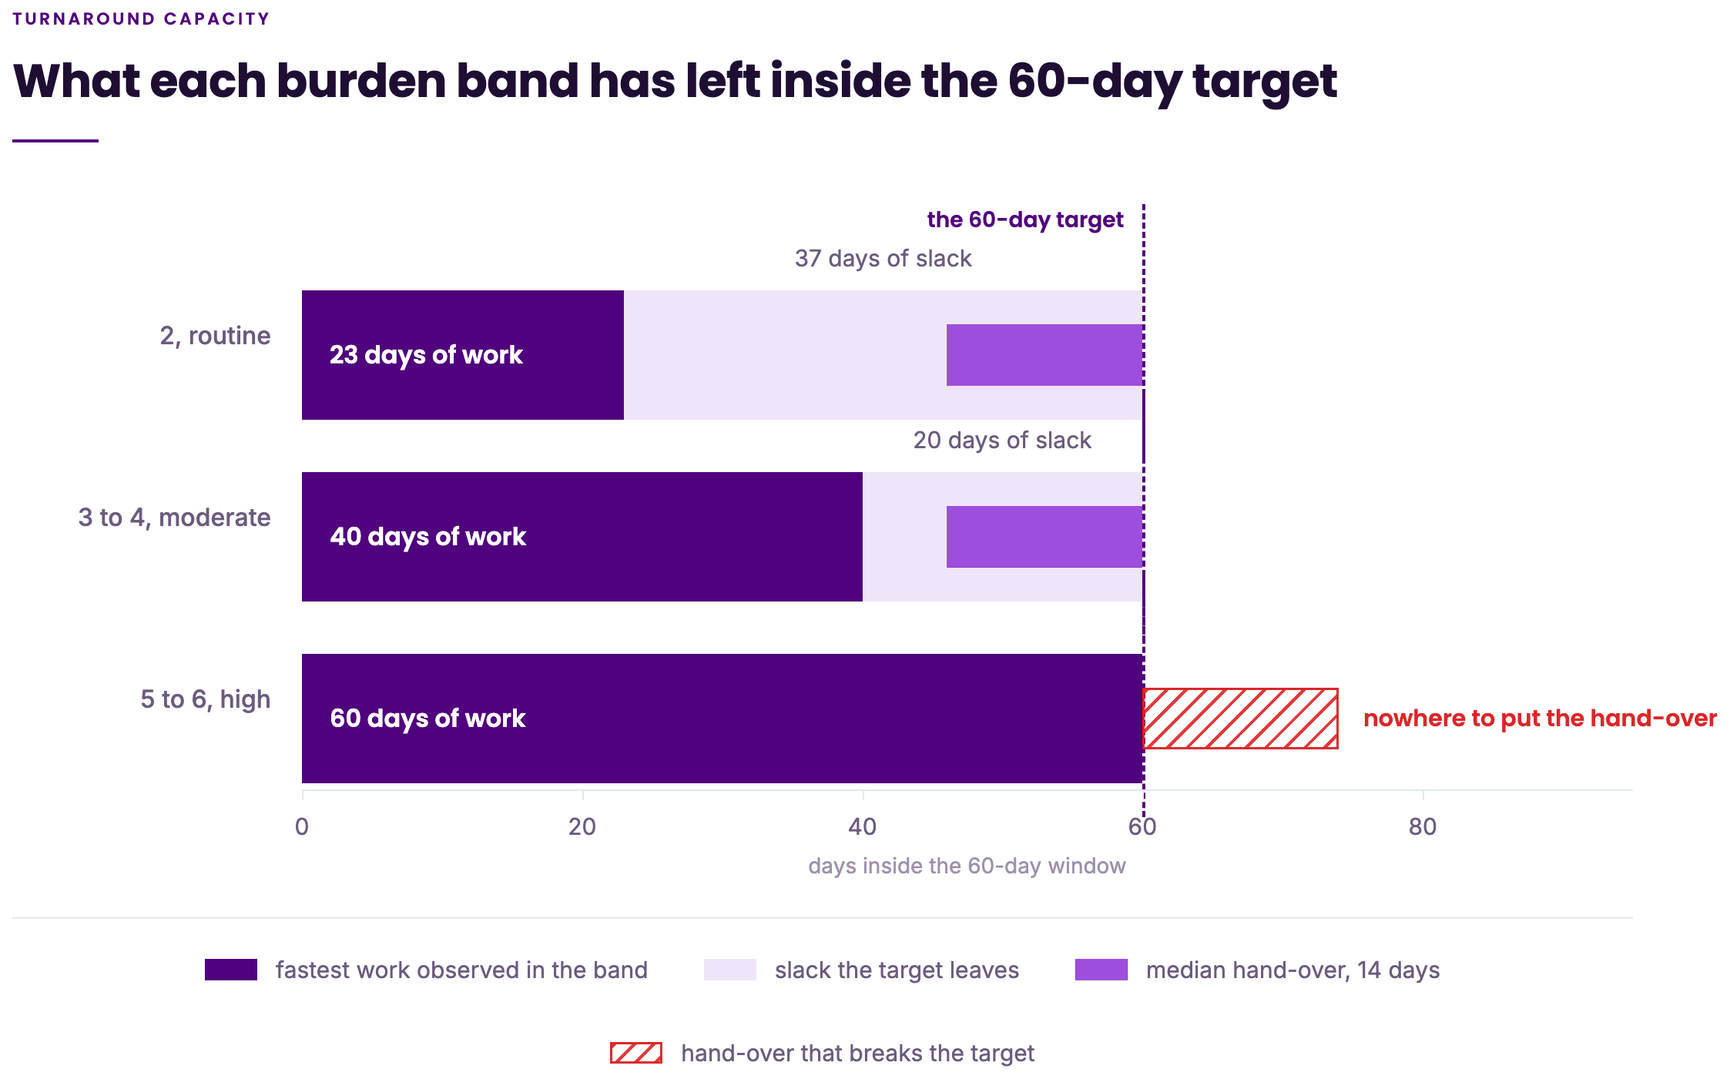
\includegraphics[width=\textwidth]{fig5_9_burden_slack.png}
  \caption{What each burden band has left inside the 60-day target}
  \label{fig:burdenslack}
\end{figure}

Preparation is the only lever these studies have, and it is not aimed at them: burden rank does not predict which trials start early (Fisher $p = 1.000$, Appendix 4.I). All six high-burden trials are aseptic, and eleven trials in the set are, so the aseptic flag identifies every one of them at notification and five others besides.

Targeting preparation at the aseptic-flagged studies concentrates effort on identifiable high-burden risk for about half the earlier notification, but its achievable on-time count is lower than preparing every committed trial, because it leaves the rescuable non-flagged trials untreated (Appendix 5.B).

The lead must be sized against the variation in durations rather than against the shortfall it closes. Appendix 5.F shows the four-day fix for BNT327-06 delivering half the time. Reading a reliability as the proportion of runs in which a plan delivers the stated outcome, a high-burden study planned at the 63-day floor is 50 per cent reliable with no lead, 75 per cent with a 28-day lead, and 90 per cent only at a 63-day lead, a second window on top of the first. Preparation is what makes a high-burden study possible; a few days of it buy a plan that says yes rather than a delivery that can be relied on.

\section{The trade-off the service faces}
\label{sec:tradeoff}

Preparation is the intervention considered here. This section reports the trade-offs it creates because the model ranks two objectives that do not always align.

The trade-off between on-time completion and weighted lateness appears only where preparation remains insufficient. On the largest queue, 1 May 2025, a 21-day lead makes each rescue cost additional lateness, whereas a 35-day lead brings two trials in on time at the lowest weighted lateness of any plan; on the 1 February 2025 queue the two objectives never conflict at any lead. Figure~\ref{fig:frontier} sets the two leads side by side and Appendix 5.C reports the frontier values.

\textbf{The conflict between finishing on time and minimising lateness is itself a symptom of insufficient preparation.} A governance rule that ranks lateness first gives up nothing when preparation is adequate and two rescues when it is not, so it is the wrong rule to fix in advance.

\begin{figure}[htbp]
  \centering
  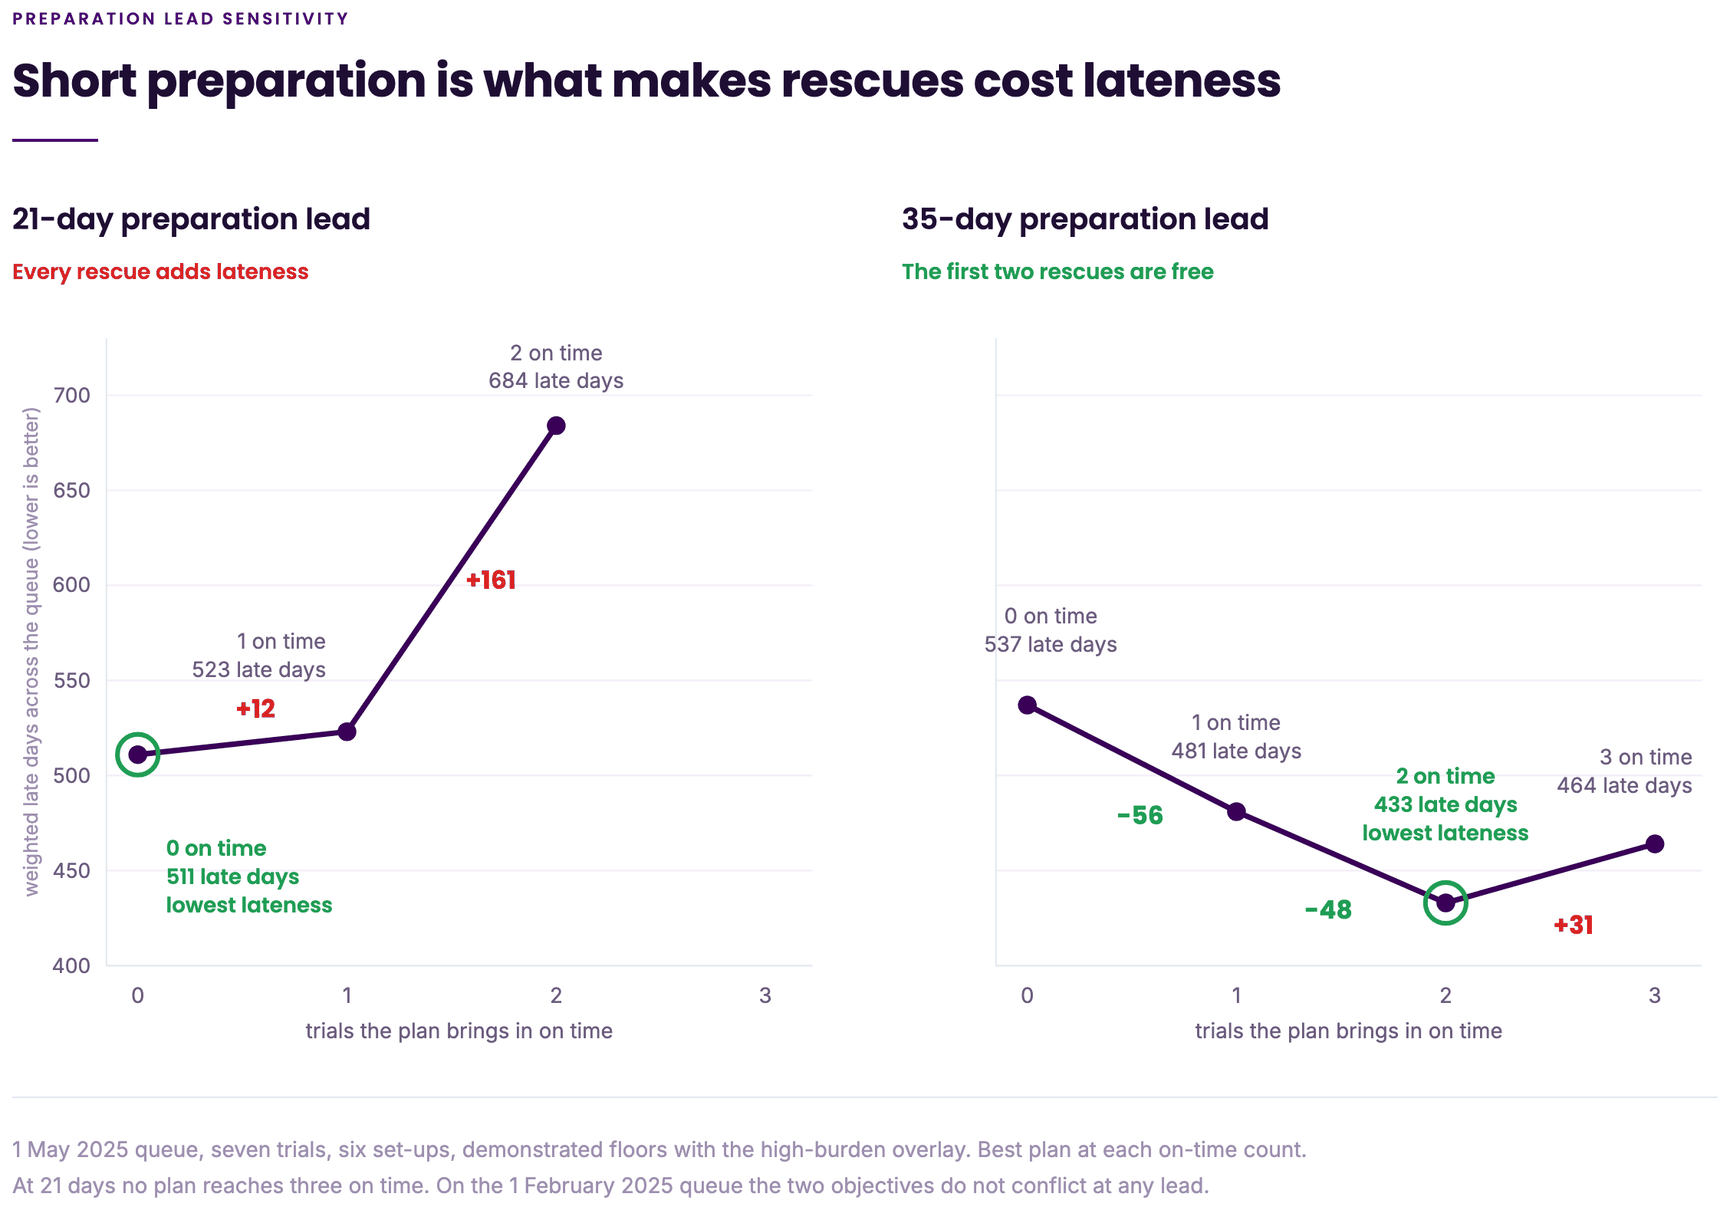
\includegraphics[width=\textwidth]{fig5_11_frontier_rotation.png}
  \caption{What a rescue costs at two preparation leads}
  \label{fig:frontier}
\end{figure}

The second trade-off is between the on-time count and the preparation it requires, the cost the trust pays in days R\&I must find. Figure~\ref{fig:prepsteps} reports the least preparation that first reaches each count.

\begin{figure}[htbp]
  \centering
  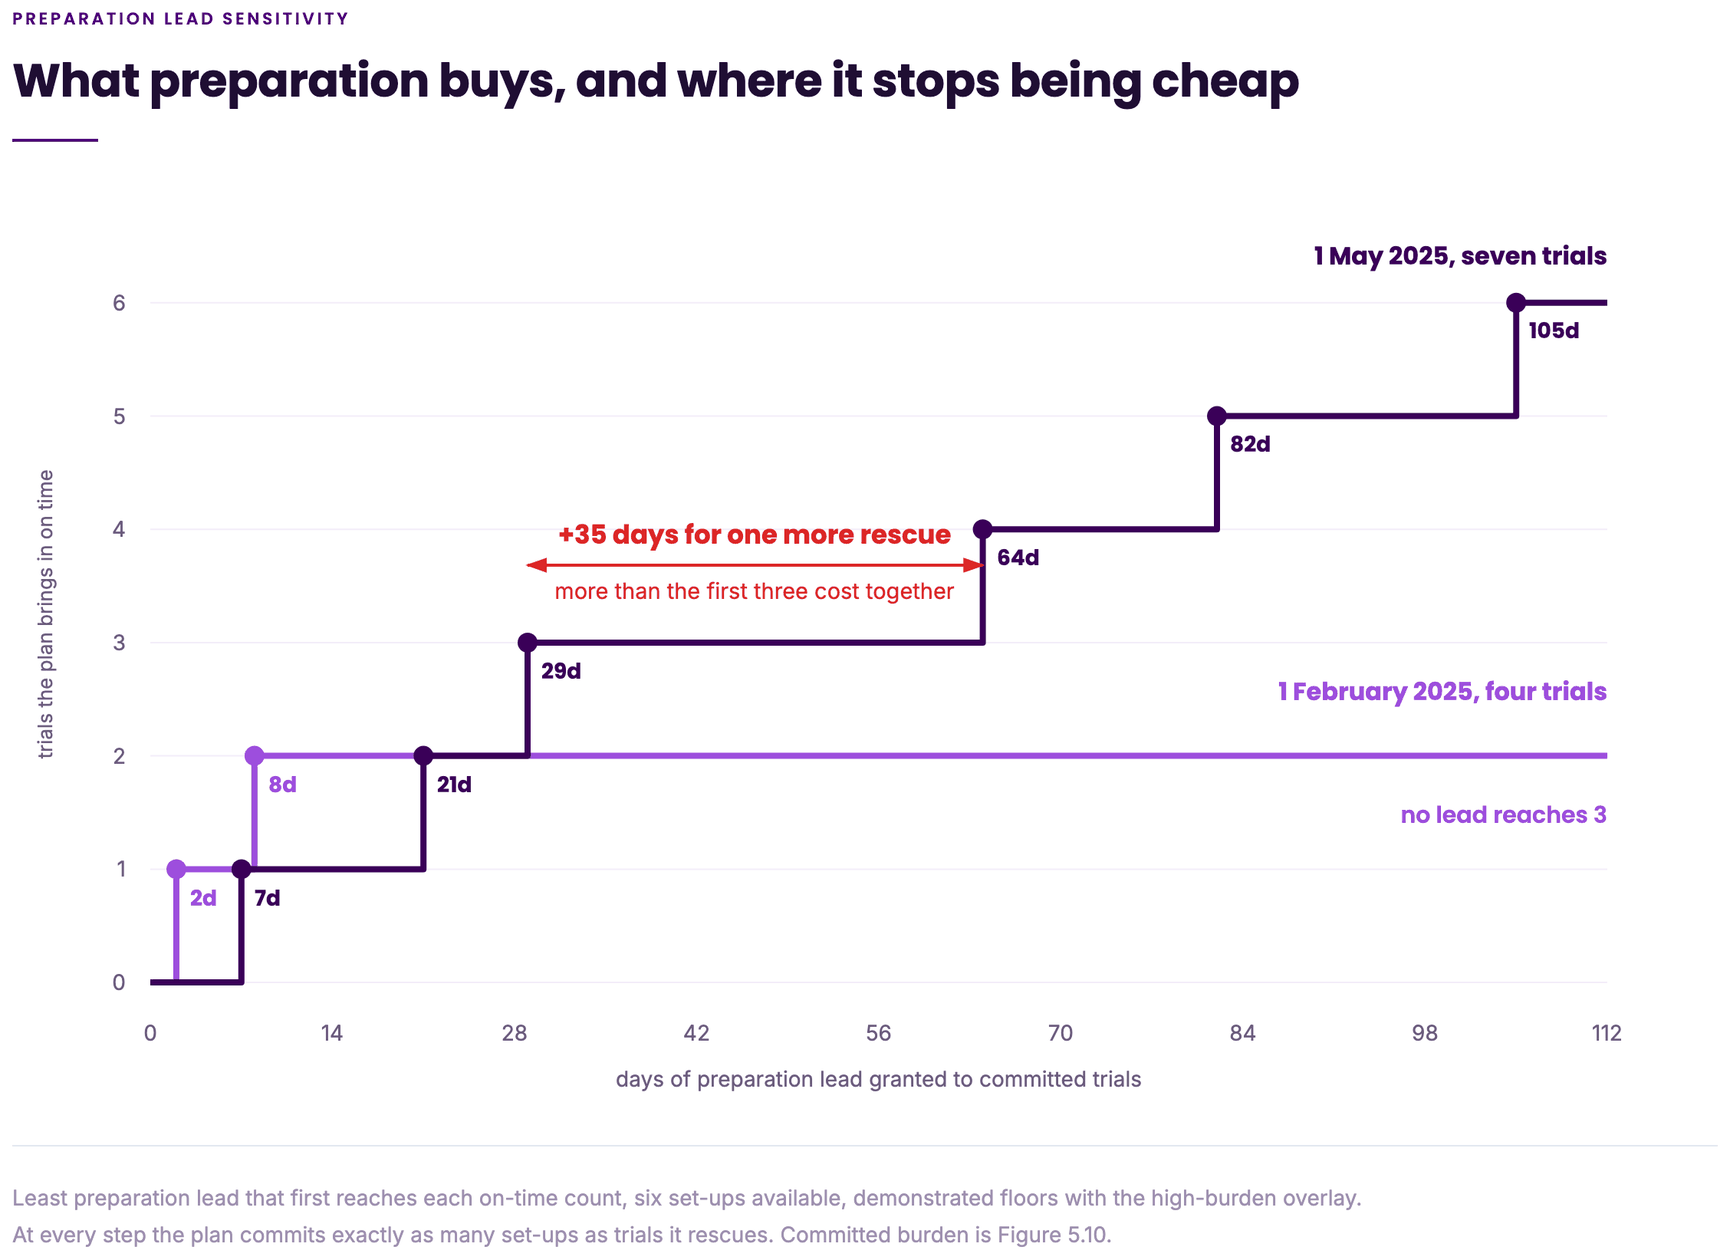
\includegraphics[width=\textwidth]{fig5_12_preparation_steps.png}
  \caption{What preparation buys, and where it stops being cheap}
  \label{fig:prepsteps}
\end{figure}

Two things follow.

First, capacity never limits the on-time count. Each rescue requires one set-up slot, so a plan that rescues three trials uses only three of the six available slots.

Second, what a queue can reach is set by its own composition. A lead only repays a shortfall the queue already carried, so it buys a rescue cheaply while a trial is near its window and buys little once a trial is far past it. Across the whole range Figure~\ref{fig:prepsteps} covers, the February queue never passes two. That ceiling belongs to the queue rather than to any lever, and it is the honest limit on what scheduling can promise.

Capacity does not stop working above the rescue count, however. Figure~\ref{fig:tradeoffpair} holds the preparation lead at 35 days and varies the set-ups opened per month against the on-time count. Lateness falls with every slot opened at each on-time count, while the pharmacy burden a plan commits rises with both. Opening more set-ups is therefore a lever on how late the rest of the queue runs rather than on how many trials meet the target. Appendix 5.C gives the values and the derived burden scale.

\begin{figure}[htbp]
  \centering
  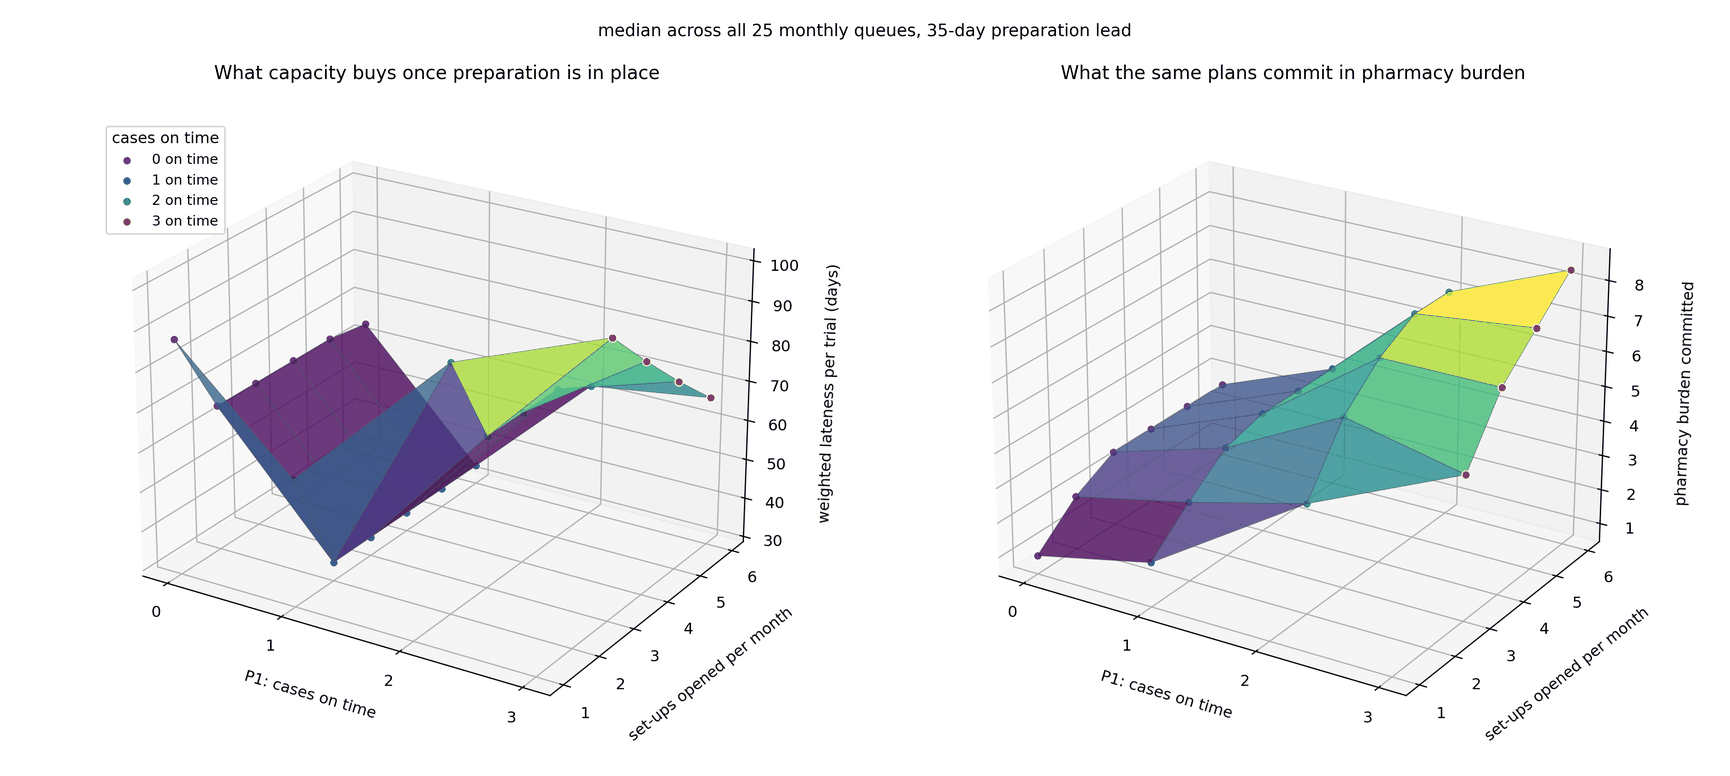
\includegraphics[width=\textwidth]{fig5_13_tradeoff_pair.png}
  \caption{What capacity buys, in days and in burden}
  \label{fig:tradeoffpair}
\end{figure}


% Chapter 6, Conclusion.
% Generated from Dissertation/Chapter6_Conclusion.md by tools/md2tex.py.
%% The draft-status line, the provenance notes and the [edit] markers in the
%% Markdown source are not part of the submitted text and are absent here.
%% Markdown is the source. Regenerate this file when it changes; do not hand-edit.

\chapter{Conclusion}
\label{ch:conclusion}
\lhead{Chapter 6. \emph{Conclusion}}

\section{Answers to the research questions}
\label{sec:answers}

Table~\ref{tab:answers} answers the critical question and its three sub-questions, and cites the evidence behind each; their full wording is in Section~\ref{sec:questions} and Table~\ref{tab:questions}.

\begin{table}[htbp]
  \centering
  \caption{Answers to the critical question and sub-questions SQ1 to SQ3*}
  \label{tab:answers}
  \begin{tabularx}{\textwidth}{@{}LL@{}}
    \toprule
    \textbf{} & \textbf{Answer} \\
    \midrule
    RQ & Four distinct trials is the maximum achievable on time across the observed decision points. The constraint is time remaining when trials reach pharmacy, not nominal capacity: high-burden set-up can consume the full 60-day window before hand-over or approval delay is considered. Preparation is therefore the only tested lever that raises the on-time ceiling, because it creates time before the clock starts. Reducing hand-over and pharmacy-queue delay improves the position of trials near the threshold, while increasing nominal capacity reduces lateness but does not create further on-time completions (Sections~\ref{sec:whythese} to~\ref{sec:levers}--5.6; Table~\ref{tab:settings}). \\
    \addlinespace
    SQ1 & Across the 25 observed decision points, only four distinct trials could be committed and completed on time within the cycle commitment limit; these trials are identified in Table~\ref{tab:fourtrials5} (Sections~\ref{sec:realqueues} to~\ref{sec:whythese}). \\
    \addlinespace
    SQ2 & Neither the cycle commitment limit nor the approval queue is the primary constraint on the on-time count. Raising the cycle commitment limit increases the on-time count at none of the 25 decision points. The limit is a maximum, so the model leaves slots unused when additional commitments would create approval delay without improving on-time performance. The binding constraint is instead the time remaining when trials reach pharmacy: extra capacity reduces lateness but does not create further on-time completions. Approval time determines usable capacity, not the on-time ceiling (Sections~\ref{sec:levers} to~\ref{sec:tradeoff}; Appendix 5.C). \\
    \addlinespace
    SQ3 & The rule improves on the arrival-order comparator only when capacity is tight: at one or two set-ups per month it can select a better committed portfolio, but from three onwards both approaches select the same trials. It therefore allocates scarce capacity rather than increasing overall performance (Section~\ref{sec:realqueues}). Its on-time advantage is not robust across simulated portfolios. It appears only at pharmacy's demonstrated duration floors, and within that regime is stronger for early arrivals and less aseptic pathway mixes. Across the demonstrated-floors regime, the rule is better in 36 per cent of runs and equal in the remainder by construction (Appendix 5.A). \\
    \bottomrule
  \end{tabularx}
\end{table}

The observed ceiling is set by usable time, not by nominal commitment capacity.

\section{Contribution and comparison with published work}
\label{sec:contrib6}

The principal contribution is the translation of LTHTR's pharmacy set-up process, existing capacity, pathways and shared approval queue into an optimisation model calibrated on the trust's records. The repeatable model makes commitment decisions explicit, compares feasible portfolios and alternative scenarios before work is committed, and assesses portfolio-level on-time performance while distinguishing nominal from usable capacity. A companion user-interface mock-up makes the model operationally interpretable: users can progressively enter trial information, identify the 60-day clock start and pathway burden, consider preparation before the clock starts, and review transparent monthly commitment recommendations.

The findings refine the practical implication of the selection literature: selection can improve the allocation of commitments and reduce lateness across the queue, but it cannot recover time lost before pharmacy receives a trial. Earlier notification and preparation therefore create the conditions in which selection can improve on-time performance (\citealp{SlotnickMorton2007OrderAcceptance}; \citealp{Munoz2018ProposalSelection}; \citealp{Qi2022EquitableEnrolment}; Sections~\ref{sec:realqueues} to~\ref{sec:levers}--5.6). Pharmacy is the first module of a wider trial set-up portfolio; comparable process, duration and capacity data from other departments would allow interdependent workstreams to be assessed jointly.

\section{Limitations}
\label{sec:limitations}

The comparison with arrival order is limited by the comparator, not by the optimisation result. The comparator is a stated rule, not a record of routine practice, which already expedites some important studies. Any reported advantage is therefore an upper bound on the benefit over current practice and limits SQ3 alone. Similarly, agreement between the model and the four trials that achieved the target is retrospective consistency rather than prospective validation (Section~\ref{sec:realqueues}; Appendix 5.A).

The four-trial ceiling is a conditional planning estimate, with its fourth on-time place particularly sensitive to the high-burden duration assumption (Section~\ref{sec:delivery}). The analysis rests on a small case-study base, estimated timing data, uncertain set-up durations and an assumed approval-time input. Sensitivity and simulation analyses test these uncertainties, but cannot independently validate the capacity ceiling or the reliability of the preparation result. In particular, holding approval delay at its expected value understates total operational uncertainty (Sections~\ref{sec:parameters} to~\ref{sec:experiments}, 5.3--5.4; Appendices 5.A and 5.C).

Preparation is not capacity-free: the base model does not charge pre-window work against the commitment limit, so it may overstate its benefit. The sensitivity analysis in Appendix 5.E shows that preparation still increases the number of decision points achieving at least one on-time completion across the tested capacity range, although the three-trial result disappears at two set-ups. Preparation is therefore a capacity-consuming intervention, not a free source of additional time.

Finally, the model selects trials for commitment but does not sequence work after commitment. The evidence therefore concerns portfolio selection only and does not establish whether a sequencing intervention could improve performance (Section~\ref{sec:notdecided}).

\section{Implications for practice and for further research}
\label{sec:implications}

The results imply four immediate actions for LTHTR: record hands-on approval time to calibrate the approval queue; flag aseptic studies at notification for targeted early preparation; plan to a reliable lower outcome rather than the deterministic maximum; and use selection to support, rather than substitute for, earlier preparation and hand-over (Sections~\ref{sec:realqueues} to~\ref{sec:delivery}--5.5).

Four research directions follow from the limitations above:

\begin{itemize}
  \item Extend the model to integrated selection and sequencing, which the present analysis cannot address.
  \item Measure pathway-specific work, approval service times and rework, so that resource use can be modelled in staff time rather than commitment counts.
  \item Optimise early preparation under finite capacity, including the activity it displaces.
  \item Prospectively evaluate the model's recommendations against observed practice, under demand growth, changing pathway mix and interdependent cross-service workflows.
\end{itemize}

---



%-----------------
%	APPENDICES
%-----------------

\addtocontents{toc}{\vspace{2em}} % Add a gap in the Contents, for aesthetics
\appendix
% Appendix A. Source: Appendix 3.A of Dissertation/Chapter3_Problem_Description.md.
% Appendix material does not count towards the word limit.

\chapter{Notation and Worked Instance}
\label{app:notation}
\lhead{Appendix A. \emph{Notation and Worked Instance}}

\section{Notation}
\label{sec:notation}

\begin{table}[htbp]
  \centering
  \caption{Notation used in the selection model of Chapter~\ref{ch:problem}}
  \label{tab:notation}
  \begin{tabularx}{\textwidth}{@{}lLl@{}}
    \toprule
    \textbf{Symbol} & \textbf{Meaning} & \textbf{Units} \\
    \midrule
    $i \in I$, $E$ & Trial awaiting pharmacy set-up; the eligible queue & n/a \\
    $G$, $due_i$ & Set-up goal (60), due day $\max(\mathrm{approval}_i, \mathrm{selection}_i) + G$ & days \\
    $p_i$ & Set-up duration of trial $i$, from its pathway & days \\
    $\delta_i$ & Days remaining to $due_i$ at the planning date, negative once breached & days \\
    $a_i$, $D$ & Days trial $i$ has waited; weight divisor (365) & days \\
    $w_i$ & Claim weight, $1 + a_i / D$ & dimensionless \\
    $c$ & Set-ups the service can commit in a cycle & trials \\
    $L$ & Planning cycle length (30) & days \\
    $g_n$ & Expected approval wait when $n$ trials are committed & days \\
    $r_{in}$ & 1 if trial $i$ finishes inside its window at committed count $n$ & binary \\
    $x_i$ & 1 if trial $i$ is committed & binary \\
    $z_n$ & 1 if the plan commits exactly $n$ trials & binary \\
    $\mathrm{onTime}_i$ & 1 if trial $i$ is committed and lands inside its window & binary \\
    $d^+_i$ & Days by which trial $i$ finishes past $due_i$ & days \\
    \bottomrule
  \end{tabularx}
\end{table}

\section{Worked instance: why on-time is a property of the plan}
\label{sec:worked}

This instance shows the mechanism Section~\ref{sec:queue} describes: the same trial can finish inside its window in a small plan and outside it in a large one, so committing more trials can leave fewer of them on time.

\textbf{Durations here are illustrative, at 36 days.} The measured durations cannot be used for this purpose. Pooled across the tracker they run to about 95 days against a 60-day window, which puts every trial outside the target whatever the plan, and removes the question the instance is meant to show. The distinction the instance makes is therefore about the model's behaviour, not about LTHTR's current position.

The expected approval wait, computed at the model's default settings, rises slowly and then sharply:

\begin{table}[htbp]
  \centering
  \caption{Expected approval wait $g_n$ at each committed count}
  \label{tab:waits}
  \begin{tabular}{@{}lrrrrrrrrr@{}}
    \toprule
    Committed count $n$ & 1 & 2 & 3 & 4 & 5 & 6 & 7 & 8 & 9 \\
    \midrule
    Wait $g_n$, days & 0.20 & 0.46 & 0.79 & 1.25 & 1.91 & 2.96 & 4.86 & 9.39 & 32.32 \\
    \bottomrule
  \end{tabular}
\end{table}

Four trials from the eligible queue, each needing 36 days of set-up, differ only in how much of their window remains:

\begin{table}[htbp]
  \centering
  \caption{The four trials of the worked instance}
  \label{tab:fourtrials}
  \begin{tabular}{@{}lrl@{}}
    \toprule
    Trial & Days remaining $\delta_i$ & Slack over the 36-day set-up \\
    \midrule
    A & 50 & 14.0 \\
    B & 44 & 8.0 \\
    C & 38 & 2.0 \\
    D & 12 & none, already short \\
    \bottomrule
  \end{tabular}
\end{table}

A trial finishes inside its window when $\delta_i \ge p_i + g_n$. Applying that at each plan size gives the rescue matrix $r_{in}$ the model reads:

\begin{table}[htbp]
  \centering
  \caption{The rescue matrix $r_{in}$ at each plan size}
  \label{tab:rescue}
  \begin{tabular}{@{}lccccccccc@{}}
    \toprule
    Plan size $n$ & 1 & 2 & 3 & 4 & 5 & 6 & 7 & 8 & 9 \\
    \midrule
    A rescueable & yes & yes & yes & yes & yes & yes & yes & yes & no \\
    B rescueable & yes & yes & yes & yes & yes & yes & yes & no & no \\
    C rescueable & yes & yes & yes & yes & yes & no & no & no & no \\
    D rescueable & no & no & no & no & no & no & no & no & no \\
    \bottomrule
  \end{tabular}
\end{table}

Three things follow, and each answers something the chapter asserts.

\textbf{Rescueability is not a property of the trial.} C survives at five committed and fails at six. Nothing about C changed; the queue it joined grew. This is why the model cannot decide trial by trial before the plan is chosen, and why the load selector $z_n$ of equation~(\ref{eq:loadselector}) exists.

\textbf{Raising the commitment limit eventually makes performance worse.} Counting trials on time as the plan grows gives three at five committed, two at six and seven, one at eight, and none at nine. The on-time count peaks and then falls, because past the peak the queue costs more days than the tightest rescueable trial has left. That is the answer SQ2 asks for, and it is why ``take every slot you can get'' is the wrong reading of a capacity case.

\textbf{A trial can be beyond help.} D has 12 days against a 36-day set-up and is outside its window at every plan size. It contributes nothing to P1 whatever the model does, which is why P2 exists: deferring D still lets its lateness grow, so the model is not free to ignore it.

Trial labels here are illustrative. The waits are computed from \texttt{Experiments/optimiser/}\allowbreak\texttt{gate.py} at default settings; the durations and remaining days are chosen to make the mechanism visible.
 % Notation and worked instance   (was Appendix 3.A)
% Appendix B. Source: Appendix 4.A of Dissertation/Chapter4_Methodology.md.

\chapter{The Tracker, its Structure and its Cleaning}
\label{app:tracker}
\lhead{Appendix B. \emph{The Tracker and its Cleaning}}

Source, unmodified: \texttt{CTIMP Trials 150 Day Metric Tracker- 2026-07-30 SE.xlsx}. Outputs: a cleaned table holding one row per trial, a model-ready extract of the fields the model uses, and the log this appendix summarises. The source file was not edited at any point, so every output is a derivative and a corrected tracker can be processed by re-running the script.

\textbf{What the tracker is.} The CTIMP 150-day metric tracker is maintained in Research and Innovation and reported against the national targets. Its Report sheet holds one row per trial across 23 columns, of which the pharmacy block runs from the day the Research Setup and Governance meeting notifies pharmacy to the day pharmacy issues its greenlight. A second sheet, Raw data, holds 2,666 rows covering the whole portfolio including declined and closed studies, and is used only to estimate the arrival rate, since studies that never reached set-up carry no pharmacy milestones.

\textbf{How the pharmacy dates get into it.} By hand, from emails, local folders and the trust's quality system, with the aseptic figures arriving separately from the Pharmacy Quality Lead. None of it is a system export, so a blank records a retrieval failure rather than an event that did not happen. Two consequences. The aseptic sign-off is a tick on a whiteboard, so there is no date to retrieve. And trials before 2023 carry only HRA approval, site selected and the open-to-recruitment date, the pharmacy fields not being collected then; since those two are the clock anchors, an old trial's deadline is computable while its duration is not.

\textbf{What the tracker does not hold.} Across the 104 distinct trials the cleaned file holds 28 pharmacy notification dates and 24 pharmacy green lights, no PPCTI sign-off dates at all, and 9 trials with no complexity tier. Figure~\ref{fig:completeness} sets every field against the rest. The gap is structural rather than random, but it does not fall where the obvious reading suggests. It tracks whether a record is held in a system, not which team owns the field. iQemo is pharmacy's own and is a digital system, and its dates are present for 51 of the 104 trials, better populated than 5 of the 9 fields arriving from outside pharmacy. The aseptic PPCTI sign-off, kept as a tick on a whiteboard, is empty for all 104. What cannot be retrieved is what was never written into a system, which is why chasing pharmacy would not have produced these dates and why the case studies were requested instead.

\begin{figure}[htbp]
  \centering
  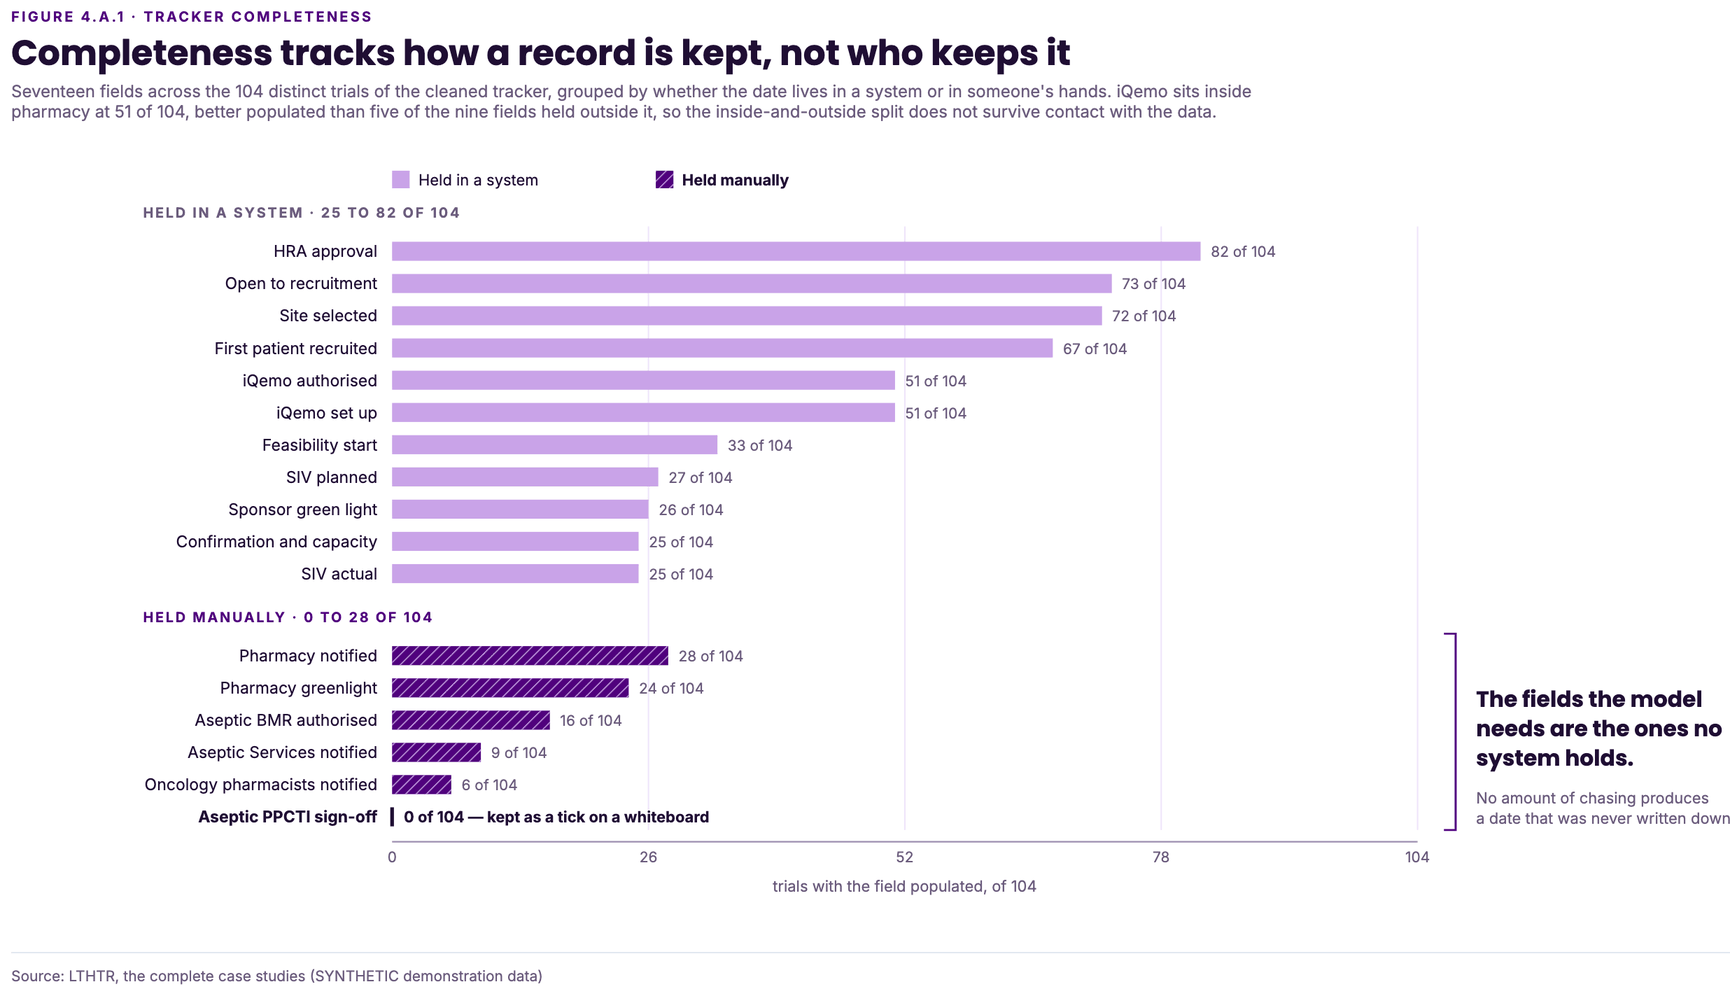
\includegraphics[width=\textwidth]{fig4_A1_tracker_completeness.png}
  \caption[Field completeness across the cleaned tracker]{Field completeness
  across the cleaned tracker, grouped by how each record is kept. Seventeen
  fields are shown against the 104 distinct trials of the cleaned file, split
  into a system-held group ranging from 25 to 82 and a manually held group
  ranging from 0 to 28. The aseptic PPCTI sign-off has no bar at all. A blank
  is a date that could not be retrieved, not a step that did not happen.}
  \label{fig:completeness}
\end{figure}

\textbf{One field reported and then set aside.} Confirmation and capacity to the \emph{sponsor's} green light has a median of exactly one day across the 23 trials holding both dates. That is not a measure of governance speed. The trust's own account is that the sponsor's green light is an announcement made once everything else is complete, so the one day measures the announcement, not the process behind it. It is a different event from the pharmacy green light of Section~\ref{sec:casestudies}, which ends set-up; the two are months apart and only the second bounds segment C. It is recorded here so that no reader treats it as evidence that governance is fast.

\begin{table}[htbp]
  \centering
  \caption{The four faults and their treatment}
  \label{tab:faults}
  \begin{tabularx}{\textwidth}{@{}LlL@{}}
    \toprule
    \textbf{Fault} & \textbf{Extent} & \textbf{Treatment} \\
    \midrule
    Trials stored as two half-filled rows & 14 pairs &
      Merged on a normalised title, each field taking the single non-empty
      value available \\
    \addlinespace
    ``As above'' in place of a date & 18 cells &
      Replaced with the value in the row above, which is what the phrase
      refers to \\
    \addlinespace
    Dates held as \texttt{dd/mm/yyyy} text & 19 cells & Parsed to real dates \\
    \addlinespace
    ``Pending'' in a date column & 4 cells &
      Left blank, since it is not a date \\
    \bottomrule
  \end{tabularx}
\end{table}

The two positional and text faults were the more damaging of the four relative to their size. All 18 ``as above'' cells and 8 of the 19 text dates sat in the pharmacy columns, so nearly the whole of both notification columns was invisible to any calculation that read them as dates.

\textbf{How the split rows were merged.} Rows were grouped on the trial title reduced to lower case with punctuation and bracketed protocol codes removed. Within a group each field took the single non-empty value available, and the longer title was kept because it carries the protocol code. Eleven of the 14 pairs merged with no conflict at all. Most apparent conflicts elsewhere were an ``as above'' against a real date, or a text date against the same date stored properly, and both dissolve once the other 2 faults are corrected.

\textbf{The three unresolved trials.} Where the two rows of a pair disagreed on a real value, the field was left blank and logged. AMPLITUDE differs by 2 to 3 years on 4 fields, with both sets internally consistent, which suggests two different studies sharing a short title rather than one split record. TAK-079-3001 differs on 3 fields, one of which looks like a transposed day and month while the others do not. Orion-BC differs by one day on a feasibility start date and affects no model quantity. Only the second costs anything: its blanked pharmacy green light removes the trial from the sample of measurable pharmacy durations.

\begin{table}[htbp]
  \centering
  \caption{What the clean-up changed}
  \label{tab:cleanup}
  \begin{tabular}{@{}lll@{}}
    \toprule
    \textbf{Quantity} & \textbf{Before} & \textbf{After} \\
    \midrule
    Distinct trials & 118 & 104 \\
    Pharmacy set-up sample & 24 & 23 \\
    Set-up median & 96 days & 95 days \\
    Set-up mean & 105.7 days & 105.9 days \\
    Within 60 days & 2 of 24 & 2 of 23 \\
    Work in progress, mean & 3.41 & 3.51 \\
    Arrival rate & 0.97 per month & 1.00 per month \\
    Trials carrying a complexity tier & 90.7 per cent & 91.3 per cent \\
    \bottomrule
  \end{tabular}
\end{table}

\textbf{An internal consistency check.} An arrival rate of 1.00 trials per month against a 95-day median sojourn implies 3.48 trials in progress by Little's Law, against 3.51 observed, a gap of 0.9 per cent. It is the only check available on the cleaned tracker that does not depend on the fields the trust cannot supply.

\textbf{What was left alone, and why.} 4 items were not repaired because repair would mean invention rather than correction: the PPCTI column, empty for all 104 trials because the step is recorded as a tick on a whiteboard; 9 trials with no complexity tier, which cannot be inferred; the sparse pharmacy dates, since cleaning cannot create a record that was never made; and the three conflicts above. The start of the 60-day clock is also untouched, being a definition rather than a data fault.
 % The tracker and its cleaning   (was Appendix 4.A)
% Appendix C. Source: Appendix 4.B of Dissertation/Chapter4_Methodology.md.

\chapter{Assumptions Behind the Approval Wait}
\label{app:queue}
\lhead{Appendix C. \emph{Assumptions Behind the Approval Wait}}

Equation~(\ref{eq:pk}) is the Pollaczek-Khinchine formula for an M/G/1 queue. The formula gives the exact long-run mean waiting time when its assumptions hold. Low utilisation reduces the size of the predicted wait. Table~\ref{tab:mg1} sets out each assumption, what it means, and how it applies to this service.

{\small
\begin{xltabular}{\textwidth}{@{}P{0.17\textwidth}>{\hsize=0.90\hsize}L>{\hsize=1.10\hsize}LP{0.17\textwidth}@{}}
  \caption{The M/G/1 assumptions checked against this service}
  \label{tab:mg1}\\
  \toprule
  \textbf{Assumption} & \textbf{What it requires} & \textbf{Evidence for this service} & \textbf{Status} \\
  \midrule
  \endfirsthead
  \toprule
  \textbf{Assumption} & \textbf{What it requires} & \textbf{Evidence for this service} & \textbf{Status} \\
  \midrule
  \endhead
  \midrule
  \multicolumn{4}{@{}r@{}}{\footnotesize\emph{continued overleaf}}\\
  \endfoot
  \bottomrule
  \endlastfoot

    Poisson arrivals &
      Work reaches the Work reaches the approver independently and is
      dispersed over time rather than arriving in batches spread out, not in
      bunches &
      A trial's clock starts at HRA approval or site selection, both set by
      the sponsor and the regulator rather than by the trust. Trials therefore
      arrive at their own pace. The fixed committees do not batch the
      signature, for the reason given below &
      Met, subject to the batching rationale below \\
    \addlinespace
    General service time &
      Only the mean and the coefficient of variation are needed &
      Pharmacy has been asked to provide direct information on approval time.
      The formula itself does not require approval times to follow a normal,
      lognormal, or other specified distribution. &
      Met \\
    \addlinespace
    Single server &
      One approver, with work queueing behind whatever they are already doing &
      The trust describes one approving person for pharmacy set-up. Pharmacy
      adds (August 2026 return) that the sign-off can be delegated to the
      operational manager when most processes are already approved &
      Approximation, conservative: a second signer can only shorten the wait \\
    \addlinespace
    Work-conserving, non-preemptive &
      The approver is never idle with work waiting, and never abandons a
      part-finished approval &
      This is consistent with the described process. It also means that the
      mean wait does not depend on the order in which trials are approved. &
      Met \\
    \addlinespace
    Unbounded queue &
      The approver does not remain idle while approval work is waiting and
      does not abandon a partly completed approval &
      Trials wait for the signature. None are abandoned for want of one &
      Met \\
    \addlinespace
    Independent service times &
      The duration of one approval does not depend on the duration of other
      approvals or on the number waiting &
      Not observable in the available records. &
      Assumed, recorded as a limitation \\
    \addlinespace
    Steady state, $\rho < 1$ &
      On average, the approver can complete work faster than new approval
      requests arrive. &
      The commitment cycle resets monthly, so the service may not fully settle
      into a long-run average. &
      Assumed, recorded as a limitation 
\end{xltabular}}


The coefficient of variation, $\kappa$, is not identified by the available records. Equation~(\ref{eq:pk}) requires the variability of pharmacy sign-off time, but no direct observations of sign-off are available. The reported model runs therefore use $\kappa = 1.55$, the coefficient of variation calculated from 51 iQemo template-build records as the most complete pharmacy-related field in the tracker. This is a temporary substitution, not a validated estimate of approval-time variability.

The iQemo measure records the time from template set-up to authorisation. Its median is 16 days, and much of that interval is likely to be time spent waiting for the template to be processed. The required approval-time measure, by contrast, concerns the duration of the signing activity itself. The proxy therefore measures a combined waiting-and-signing interval rather than signing time alone.

The direction of the error cannot be established. The observed interval combines waiting and signing time, and adding waiting can change both the mean and the variance. Consequently, the coefficient of variation of the combined interval may be lower than, similar to, or higher than the coefficient of variation of signing alone.

This depends on the relative variability of waiting and signing time, and on whether they move together. Neither is identified in the records. Independence cannot be tested and should not be assumed.

The central problem is identification. The 16-day iQemo interval combines waiting and signing, but the available data do not separate those components. Its coefficient of variation therefore does not identify the coefficient of variation of signing time. The true signing-time $\kappa$ could be lower than, close to, or higher than 1.55. The proxy consequently places little constraint on $\kappa$.

The value is retained solely to allow equation~(\ref{eq:pk}) to be evaluated while direct pharmacy sign-off data are unavailable. It is not treated as an estimate of signing-time variability, and no substantive conclusion in this thesis depends on $\kappa = 1.55$ being accurate.

The observed proxy may not vary in the same way as sign-off time. Direct sign-off observations would be needed to test whether the two are comparable. Pharmacy has therefore been asked for its quickest, usual, and longest hands-on sign-off times. These responses will define plausible bounds rather than provide an exact estimate, and the model will test gate waiting time across those bounds.

Pharmacy's three responses give a minimum-to-maximum range. However, equation~(\ref{eq:pk}) requires the coefficient of variation, $\kappa$, which depends on both the mean and the standard deviation. A range measures the distance between the extremes, not the typical spread of observations around the mean. the range must be converted into an approximate standard deviation before $\kappa$ can be estimated.

Hartley's $d_2$ provides a standard way to convert the range of a normal sample into an estimated standard deviation. Dividing by four is a practical approximation when the range represents roughly 25 observations. Approval times are unlikely to be normally distributed, so this is a convenience assumption rather than a claim about their true distribution. It is used because the available evidence consists only of three broad response from the LTHTR.

Chapter~\ref{ch:results} currently uses $\kappa = 1.55$, because the pharmacy response was not available when the model runs were produced. Once the response is received, the model will be rerun at both ends of the plausible $\kappa$ interval. If the capacity conclusion does not change, the substitution has not affected the result. If it does change, this will show that the conclusion is sensitive to variation in an approval process that the service has not yet measured.

The conversion has three main limitations. First, if approval times are right-skewed, a normal-based conversion may be misleading. Second, the number of observations behind the recalled quickest and longest times is unknown. Third, in a skewed distribution, the range may not be symmetric around the mean. A fitted lognormal or gamma distribution would be preferable, but this would require actual sign-off observations rather than three recalled bands.

A separate unresolved input is $A$, approver availability per cycle (capacity). It is held fixed because the trust has not supplied the required information, and this assumption is documented in Section~\ref{sec:parameters}.

DEAS and GMO committees release studies in batches, which might be conflicted with the model's arrival assumption. However, approval occurs after a long and variable set-up period. That period disperses studies from each committee batch across later months, so much of the original batch pattern is lost before studies reach the approval gate.

This reasoning depends on approval occurring near the end of set-up. It also does not mean that the 95-day duration and the $\kappa$ estimate should be treated as parameters from the same distribution: they are drawn from different samples and should remain separate.
 % Approval-wait assumptions      (was Appendix 4.B)
% Appendix D. Source: Appendix 4.C of Dissertation/Chapter4_Methodology.md.

\chapter{What the 52 Automated Tests Check}
\label{app:tests}
\lhead{Appendix D. \emph{What the 52 Automated Tests Check}}

Section~\ref{sec:verification} reports 52 tests. This appendix says what each one checks, so the count can be verified and any single check found. Every test runs whenever the code changes, and a failing test stops the change rather than reporting the problem afterwards.

\section{The selection model, tests 1 to 35}
\label{sec:testsmodel}

The model of Chapter~\ref{ch:problem}, and the two refinements of Section~\ref{sec:parameters}.

\begin{longtable}{@{}rp{0.86\textwidth}@{}}
  \caption{Tests 1 to 13: the selection model}
  \label{tab:tests1}\\
  \toprule
  & \textbf{The test checks that} \\
  \midrule
  \endfirsthead
  \toprule
  & \textbf{The test checks that} \\
  \midrule
  \endhead
  \bottomrule
  \endfoot
  1  & The demonstration instance loads with 16 trials covering all four pathways \\
  2  & The demonstration durations are short enough to show the on-time mechanism, which the measured durations are not \\
  3  & The solver finds the same plan as checking every possible plan one at a time \\
  4  & The solver agrees with the simpler ranking rule wherever that rule is known to be correct \\
  5  & No plan commits more trials than the limit allows \\
  6  & The model commits fewer trials than the limit when an extra trial would cost a rescue \\
  7  & Ranking on lateness alone rescues no trial, which is why on-time is ranked first \\
  8  & Putting on-time first never improves lateness; it can only cost lateness \\
  9  & A study scoring below the value floor is closed rather than left in the queue \\
  10 & An empty queue returns a plan rather than an error \\
  11 & The capacity check made before solving agrees with what the solver returns \\
  12 & A trial that cannot be planned is returned marked as blocked, not quietly dropped \\
  13 & Solving through the planner interface gives the same plan as using the model directly \\
\end{longtable}

\begin{longtable}{@{}rp{0.86\textwidth}@{}}
  \caption{Tests 14 to 17: the withdrawn trade setting}
  \label{tab:tests2}\\
  \toprule
  & \textbf{The test checks that} \\
  \midrule
  \endfirsthead
  \toprule
  & \textbf{The test checks that} \\
  \midrule
  \endhead
  \bottomrule
  \endfoot
  14 & The withdrawn setting has been removed from the model, not merely set to zero \\
  15 & A request still using it is refused rather than silently given an unchanged plan \\
  16 & Switching the value objective on never costs an on-time trial \\
  17 & Portfolio value rises with the commitment limit, which is why trading a trial away never pays \\
\end{longtable}

\begin{longtable}{@{}rp{0.86\textwidth}@{}}
  \caption{Tests 18 to 23: segment B, the days lost before a trial reaches pharmacy}
  \label{tab:tests3}\\
  \toprule
  & \textbf{The test checks that} \\
  \midrule
  \endfirsthead
  \toprule
  & \textbf{The test checks that} \\
  \midrule
  \endhead
  \bottomrule
  \endfoot
  18 & A trial already in pharmacy's queue does not lose the same days twice \\
  19 & A trial not yet handed over loses the days before hand-over \\
  20 & A trial R\&I still holds is planned on the median hand-over and marked as assumed \\
  21 & A trial with no usable dates is blocked rather than given an invented window \\
  22 & Subtracting the hand-over can cost a trial its rescue, which is the point of the correction \\
  23 & An assumed hand-over is always reported as assumed, never as a recorded date \\
\end{longtable}

\begin{longtable}{@{}rp{0.86\textwidth}@{}}
  \caption{Tests 24 to 35: segment A, the preparation credit}
  \label{tab:tests4}\\
  \toprule
  & \textbf{The test checks that} \\
  \midrule
  \endfirsthead
  \toprule
  & \textbf{The test checks that} \\
  \midrule
  \endhead
  \bottomrule
  \endfoot
  24 & With no credit set, every plan matches the plan produced before the credit existed \\
  25 & With both conditions met, the credit shortens the set-up \\
  26 & Complexity alone earns nothing without the sponsor green light \\
  27 & The green light alone earns nothing without complexity \\
  28 & A Phase 1 study earns the credit without needing aseptic work \\
  29 & Every input to the credit comes from the data request; none is invented \\
  30 & The planner can add a study the rule would miss \\
  31 & The planner can withhold the credit from a study the rule would give it to \\
  32 & The planner cannot waive the sponsor green light \\
  33 & The credit never shortens a study below one day \\
  34 & A negative credit is refused \\
  35 & The credit can turn a missed deadline into a rescue \\
\end{longtable}

\section{The robustness experiment, tests 36 to 40}
\label{sec:testsrobust}

Tests 36 and 37 are the two hand-worked checks of Section~\ref{sec:verification}.

\begin{longtable}{@{}rp{0.86\textwidth}@{}}
  \caption{Tests 36 to 40: the robustness experiment}
  \label{tab:tests5}\\
  \toprule
  & \textbf{The test checks that} \\
  \midrule
  \endfirsthead
  \toprule
  & \textbf{The test checks that} \\
  \midrule
  \endhead
  \bottomrule
  \endfoot
  36 & The four-trial instance of Appendix~\ref{app:notation} gives the same answer worked by hand and computed by the model \\
  37 & The lateness calculation matches equation~(\ref{eq:lateness}) worked by hand \\
  38 & A scenario regenerates exactly from its seed \\
  39 & The comparator commits the longest-waiting trials, as Section~\ref{sec:comparison} describes \\
  40 & Checking every plan one at a time and solving directly return the same plan \\
\end{longtable}

\section{The plan-level uncertainty run, tests 41 to 52}
\label{sec:testsuncertainty}

Tests 41 to 43 fix the run's agreement with the plan it qualifies.

\begin{longtable}{@{}rp{0.86\textwidth}@{}}
  \caption{Tests 41 to 52: the plan-level uncertainty run}
  \label{tab:tests6}\\
  \toprule
  & \textbf{The test checks that} \\
  \midrule
  \endfirsthead
  \toprule
  & \textbf{The test checks that} \\
  \midrule
  \endhead
  \bottomrule
  \endfoot
  41 & With no variation in duration, the run returns the planning model's on-time count exactly \\
  42 & With variation, the promised count is not always achieved, which is the point of the run \\
  43 & Only the set-up spread widens the drawn durations; the approval-time figure cannot \\
  44 & The reported distribution adds to one and never exceeds the number of trials committed \\
  45 & The pessimistic figure never reads higher than the average \\
  46 & The trial most likely to miss its deadline is reported first \\
  47 & A trial the plan cannot rescue is never shown as rescued \\
  48 & A larger plan carries a longer approval wait \\
  49 & A run repeats exactly from the same seed \\
  50 & A different seed gives a different result \\
  51 & An empty plan is refused \\
  52 & A run must have at least one repetition \\
\end{longtable}
 % The 52 automated tests         (was Appendix 4.C)
% Appendix F. Source: Appendix 5.A of Dissertation/Chapter5_Results.md.

\chapter{The Robustness Sweep}
\label{app:sweep}
\lhead{Appendix \thechapter. \emph{The Robustness Sweep}}

The sweep tests one narrow question: does the selection rule's advantage survive when arrival timing, pathway mix and set-up duration are varied? It does not test preparation or the hand-over correction, and it runs on generated portfolios rather than on the trust's own queues.

\begin{table}[htbp]
  \centering
  \caption{The scenario grid}
  \label{tab:grid}
  \begin{tabularx}{\textwidth}{@{}P{2.9cm}P{4.4cm}L@{}}
    \toprule
    \textbf{Axis} & \textbf{Values} & \textbf{Grounding} \\
    \midrule
    Arrival timing & early, typical, late &
      Days remaining at the planning date, spanning the tracker's observed spread \\
    \addlinespace
    Aseptic share & 0.4, 0.6, 0.8 &
      Centred on the trust's own 60\% figure \\
    \addlinespace
    Prescription share & 0.2, 0.4 &
      No trust figure exists, so it is varied rather than assumed \\
    \addlinespace
    Duration regime &
      calibrated at 0.8, 1.0 and 1.2 times the case-study medians; the
      Appendix 4.H floors; the pooled 62-day figure &
      Current performance, demonstrated performance, and the achievable pooled
      quantile \\
    \bottomrule
  \end{tabularx}
\end{table}

90 cells, 100 portfolios each, 9,000 in total, one fixed seed per cell.

\begin{table}[htbp]
  \centering
  \caption{On-time wins against the arrival-order rule, by duration regime}
  \label{tab:sweepwins}
  \begin{tabular}{@{}lrrr@{}}
    \toprule
    \textbf{Regime} & \textbf{Wins} & \textbf{Draws} & \textbf{Win rate} \\
    \midrule
    Calibrated, 0.8$\times$ & 0 & 1,800 & 0\% \\
    Calibrated             & 0 & 1,800 & 0\% \\
    Calibrated, 1.2$\times$ & 0 & 1,800 & 0\% \\
    \textbf{Floors}        & \textbf{640} & \textbf{1,800} & \textbf{36\%} \\
    Pooled 62 days         & 0 & 1,800 & 0\% \\
    \bottomrule
  \end{tabular}
\end{table}

The finding is that the rule has no advantage of its own. Four of the five duration regimes return exactly zero wins in 1,800 draws each: current performance, current performance 20\% faster, current performance 20\% slower, and the pooled 62-day figure. The rule gains something in one regime only, the durations pharmacy has already demonstrated, and there it wins 36\% of the time. An advantage that appears in one of five regimes and vanishes in the other four is a property of the queue, not of the ordering.

The other two axes say which queues those are. The rule wins in 75\% of draws when trials arrive early, 32\% at the typical arrival time and never in any of the 600 draws where they arrive late, which is the same result Section~\ref{sec:whythese} reads off the real queues: a trial that reaches pharmacy after most of its window has gone cannot be recovered by any ordering. Its wins also fall from 45\% to 24\% as the aseptic share rises from 0.4 to 0.8. The trust's own mix of roughly 60\% aseptic sits between them, at 38\%, and the direction of travel is towards the heavier end.

Three things follow. First, selection is the third lever rather than the first. A service that adopts this rule without changing durations gains nothing, and the four zero rows are what that looks like measured; Section~\ref{sec:levers} reaches the same ordering from the real queues by finding preparation and the two delays ahead of any scheduling change. Second, the rule is a rationing device rather than an improvement. Section~\ref{sec:realqueues} finds its advantage on the real queues at one and two set-ups a month and gone from three, so it earns its keep exactly where capacity is tightest and stops mattering once capacity is not, which is the opposite of how a scheduling tool is usually sold. Third, each win is bought. The 640 wins cost 24.3 weighted days of lateness elsewhere apiece, so the rule trades delay across the queue for a threshold rather than removing delay, which is the Section~\ref{sec:tradeoff} trade-off appearing again on generated data.

\textbf{Three limits.} The model never loses, which is by construction rather than a finding: it attains the maximum achievable on-time count, so a loss is impossible. The 36\% is therefore 36\% better and 64\% identical, not a rule that is worse the rest of the time. The generator draws studies already queued, so the sweep cannot exercise preparation and understates it throughout. And the comparator, committing the longest-waiting study first, is more mechanical than real practice, which already accelerates studies judged important; any advantage shown here is therefore an upper bound.
 % The robustness sweep           (was Appendix 5.A)
% Appendix G. Source: Appendix 5.B of Dissertation/Chapter5_Results.md.

\chapter{Targeted Against Untargeted Preparation}
\label{app:targeted}
\lhead{Appendix \thechapter. \emph{Targeted Against Untargeted Preparation}}

Section~\ref{sec:levers} reports that preparation aimed only at high-burden studies reaches almost as many dates for about half the earlier notification. This is the sweep behind that sentence.

The regime matches Table~\ref{tab:settings}: the strict anchor rule, the demonstrated floors, the high-burden overlay at 63 days, six slots, and the same twenty-five decision points. Targeted preparation grants the lead only to committed trials in burden band 5 or 6. Spread preparation grants it across the queue.

\begin{table}[htbp]
  \centering
  \caption{What each lead reaches, targeted against spread}
  \label{tab:targeted}
  \small
  \setlength{\tabcolsep}{4pt}
  \begin{tabular}{@{}lrrrrrrrr@{}}
    \toprule
    & \multicolumn{4}{c}{\textbf{Targeted}} & \multicolumn{4}{c}{\textbf{Spread}} \\
    \cmidrule(lr){2-5}\cmidrule(l){6-9}
    \textbf{Lead} & \textbf{$\geq 1$} & \textbf{$\geq 2$} & \textbf{Best} & \textbf{R\&I days}
                  & \textbf{$\geq 1$} & \textbf{$\geq 2$} & \textbf{Best} & \textbf{R\&I days} \\
    \midrule
    0 days  & 9 of 25  & 0 & 1 & 0     & 9 of 25  & 0  & 1 & 0 \\
    7 days  & 10 of 25 & 0 & 1 & 147   & 11 of 25 & 0  & 1 & 469 \\
    14 days & 11 of 25 & 0 & 1 & 294   & 12 of 25 & 2  & 2 & 980 \\
    21 days & 12 of 25 & 0 & 1 & 441   & 14 of 25 & 4  & 2 & 1,407 \\
    35 days & 14 of 25 & 1 & 2 & 735   & 18 of 25 & 7  & 3 & 2,450 \\
    60 days & 16 of 25 & 2 & 2 & 1,260 & 20 of 25 & 12 & 3 & 4,020 \\
    \bottomrule
  \end{tabular}
\end{table}

Read the table across equal counts rather than equal leads. Twelve dates cost 441 trial-days of earlier notification when the lead is targeted and 980 when it is spread; fourteen dates cost 735 against 1,407. Roughly half the R\&I effort reaches the same number of dates.

The ceiling is what targeting gives up. It never reaches three trials on time, and reaches two at only two dates, against three and twelve when the lead is spread. Not every rescuable trial is a heavy one, so a lead confined to bands 5 and 6 cannot reach the trials that the spread lead rescues.

Every figure comes from \texttt{analyse\_burden\_and\_preparation}. Its untargeted arm reproduces the preparation row of Table~\ref{tab:settings} exactly, 20 of 25 dates at a 60-day lead, which is what makes the two arms comparable.
 % Targeted vs untargeted prep    (was Appendix 5.B)
% Code listings stub from the original template. Uncomment when you need it.
%\chapter{Code Listings}
\label{AppendixA}
\lhead{Appendix A. \emph{Code Listings}}

\todo{Include a full listing of all your code you have written for the project. If your project involves modifying code previously written by others, then you may include this other code as long as you indicate clearly in the code listing what parts have been written by you.
%
Example is provided below:
}

\begin{lstlisting}[language = Java]
import java.util.*;
import java.util.ArrayList;
import java.util.Random;
import java.util.List;

public class SRIE {
}

\end{lstlisting}

\addtocontents{toc}{\vspace{2em}} % Add a gap in the Contents, for aesthetics
\backmatter
\label{Bibliography}
\lhead{\emph{Bibliography}}
\bibliographystyle{unsrtnat}
\bibliography{Ref}

\end{document}
